
\chapter{Susceptibilidad magnética} % Main chapter title



\begin{center}

. . . . .Todo lo que usted quiera, concluyó un convidado, \\
pero si no cree en el magnetismo después de eso, \\
¡es usted un ingrato, mi querido señor!


\hspace{5.6cm} Magnetismo\\
\hspace{4.6cm} Guy
de maupassant  
\end{center}


\vspace{0.5cm} 

\section{susceptibilidad magnética} 
El campo magnético dentro de una sustancia se lo llama inducción magnética $\V{B}$ y difiere del campo magnético en el vacío $\V{H}$. La diferencia es el aporte del medio material llamado magnetización $\V{M}_{0}$ momento dipolar inducido por unidad de volumen

\begin{equation*}
\V{B}= \V{H} + 4\pi\V{M}\; \text{CGS} \qquad  \V{B}= \mu_{0}(\V{H} +\V{M})\; \text{SI}
\end{equation*}

Donde $\mu_{0}$ es la permeabilidad magnética del vacío. La relación entre $\V{M} \left[ \dfrac{a}{m} \right]$ Y $\V{h} \left[ \dfrac{a}{m} \right]$ se llama susceptibilidad magnética por unidad de volumen $\chi_{V}$ y es adimensional:

\begin{equation*}
\chi_{V} = \dfrac{\vert\V{M}\vert}{\vert\V{H}\vert}
\end{equation*}

También se puede escribir $\V{B}= \mu_{0}(\V{H} + \V{M}) = \mu_{0}(\V{H} + \chi_{v}\V{H}) = \mu_{0}(1 + \chi_{v})\V{H} = \mu \V{H}$ donde $\mu$ es la permeabilidad magnética.

La susceptibilidad $\chi_{v}$ es análoga a la $\chi_{e}$ llamada susceptibilidad eléctrica y en ambos casos miden la respuesta del medio al campo magnético externo o al campo eléctrico externo También es usada la susceptibilidad magnética molar $\chi=V_{m}\chi_{v}$ donde $V_{m}$ es el volumen molar. Si la magnetización de la muestra aumenta, la susceptibilidad magnética es positiva y si disminuye es negativa. La susceptibilidad magnética se medida por la balanza de Gouy\footnote{La balanza de Gouy, inventada por el físico francés Louis Georges Gouy (1854-1926), mide la susceptibilidad magnética de una muestra, a través de su atracción o repulsión por un gradiente de campo magnético. La muestra se introduce en un recipiente cilíndrico alargado, suspendido de una balanza y penetrando parcialmente entre los polos de un imán. La balanza mide el cambio de masa aparente al ser repelida o atraída por la región de alto campo magnético entre los polos. Este método es de importancia histórica, de interés didáctico y permite determinaciones susceptométricas a un coste muy bajo. En la actualidad es común el uso de métodos mucho más sensibles como los magnetómetros dotados de SQUID}.

La susceptibilidad magnética permite clasificar a los materiales de acuerdo al comportamiento de la sustancia frente a un campo magnético externo Pueden ser clasificados en los siguientes casos (por ahora en estos dos): 

\begin{itemize}
\item Diamagnéticos: tienen susceptibilidad $\chi_{v}<0$

\item Paramagnéticos: tienen susceptibilidad  $\chi_{v}>0$
\end{itemize}

El paramagnetismo y el diamagnetismo fueron descubiertos por Faraday. Lo expuesto es una de las manera de definir paramagnetismo y diamagnetismo. No hay sustancias para las cuales  $\chi_{v}=0$. en el caso de que  $\chi_{v}<0$ entonces  $\V{B}=0$ y estaremos en presencia de un {\color{red} material diamagnético ideal} de tal manera que expulsa
al campo $\V{B}$ fuera del cuerpo, luego es un superconductor.

La clasificación del magnetismo en los sólidos de la figura \ref{fig:s0} no pretende ser completa. No incluimos moléculas, iones y compuestos químicos y otros casos más. Pero, pese a estas limitaciones, creo que didácticamente se justifica y da una idea de lo vasto del tema.

\begin{figure}[H]
    \centering
    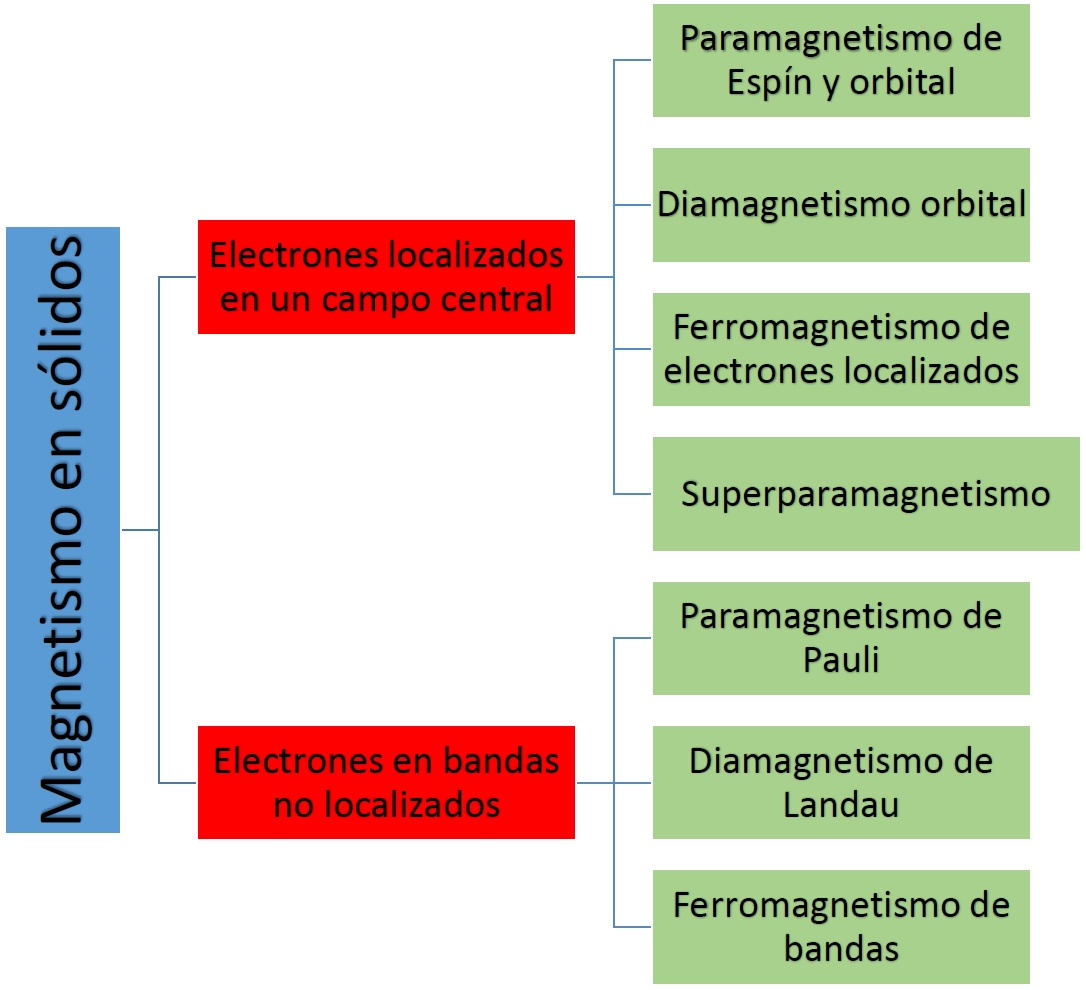
\includegraphics[width=0.8\textwidth]{./Figures/fig_s0}
	\caption{Magnetismo en sólidos}
	\label{fig:s0}
\end{figure}

\subsection{Paramagnetismo atómico}

\begin{itemize}

\item Todos los átomos y moléculas que tienen un momento magnético son paramagnéticos.

\item En un átomo tanto el momento de spin como el angular aportan al paramagnetismo aunque generalmente el aporte del espín es más importante.

\item Por tanto los átomos con capas externas completas tienen momento magnético cero,cero,(gases inertes pero también Zn, Cd, Hg los elementos con solo electrones $s$ no tienen momento orbital $l=0$ en estos casos el momento magnético atómico se debe solo al spin Los alcalinos con un solo electrón en la capa $s$ tienen un momento magnético de un magnetón, lo mismo es cierto para el (Ag, Au).

\item En átomos con niveles completamente ocupados, los momentos magnéticos se compensan y no hay momento magnético resultante.

\item  El momento magnético de espín puede estar en dirección paralela al campo exterior o antiparalela a éste.

\item Son paramagnético todos los átomos y moléculas que poseen un número impar de electrones, pues presentan un momento magnético El spin total del sistema no debe ser nulo, Ejemplo átomos libres de sodio, oxido nítrico gaseoso ($NO$).

\item También son paramagnéticos todos los átomos y iones libres con una capa interna incompleta, ejemplo elementos de transición, $Mn^{2+}, \; Gc^{3+}$.

\item Todas las sustancias a altas temperaturas son o bien diamagnéticas o bien paramagnéticas.

\item El momento magnético fundamental es el magnetón de Bohr ($\mu_{B}$) que tiene una magnitud de $9,27\times 10^{-24}\left[A\; m^{2} \right]$. Para cada electrón en el átomo el momento magnético de espín es $\pm\mu_{B}$ la contribución del momento magnético de orbital es igual a $m_{l}\mu_{B}$ con $m_{l}$ el número cuántico magnético del electrón.


\item Por ultimo aquellos que tienen una capa interna no completa poseen un momento magnético importante (elementos de transición), estos son los casos que nos interesa Como ya mencionamos los elementos de transición tienen el momento orbital bloqueado.

\end{itemize}

\subsection{Paramagnetismo cuántico}

En este tema no hay mucho mas que hablar la mayoría de las ideas ya las hemos formulados. Se vio que el momento magnético total del átomo sin considerar el núcleo es:

\begin{equation}
\V{\mu}_{total}= \V{\mu}_{L}+\V{\mu}_{S}=-\mu_{B}(\V{L}+g_{e}\V{S})= =-\mu_{B}(\V{L}+2\V{S})=-\mu_{B}(\V{J}+\V{S}) 
\end{equation}

%Tomemos un ejemplo realizado anteriormente y trabajamos en \textbf{unidades del magnetón de Bohr}: supongamos $l=1$ y como

\begin{equation*}
  \vert 1 - \dfrac{1}{2} \vert \leq j \leq  \vert 1 + \dfrac{1}{2} \vert \rightarrow \dfrac{1}{2}; \dfrac{3}{2}
\end{equation*}

Luego tomamos $j=\dfrac{1}{2}$ entonces:

\begin{equation*}
  |\V{J}|=\sqrt{\dfrac{1}{2}\big(\dfrac{1}{2}+1\big)}=\sqrt{\dfrac{3}{4}}=0,86; \; |\V{L}|=\sqrt{1(2)}=\sqrt{2}=1,41;\; |\V{S}|=\sqrt{\dfrac{1}{2}\big( \dfrac{3}{2} \big)}= \sqrt{\dfrac{3}{4}}=0,86
\end{equation*}

Como se vio el ángulo entre $l$ y $s$ se calcula por

\begin{equation*}
	Cos(\alpha) = \dfrac{j(j+1)-l(l+1)-s(s+1)}{2\,\sqrt{l(l+1)}\,\sqrt{s(s+1)}}
\end{equation*}

y en nuestro caso da apróximadamente $145^{o}$

Calculemos ahora los momentos \textbf{magnéticos en unidades de $\mu_{B}$}

\begin{equation*}
  \lv{\mu_{L}}= \qa{l}= \lv{L};\quad \lv{\mu_{S}}=2\qa{s}=2\lv{S}
\end{equation*}

$\lv{\mu_{j}}=g_{i}\lv{J}$ o bien $\lv{\mu_{j}}=|\V{mu}_{total}|Cos(\Theta)$ Recordando que:

\begin{equation*}
	g_{j}= 1 +\dfrac{\qa{l}+\qa{s}-\qa{l}}{2\qa{j}} \quad \text{como veremos seguidamente}
\end{equation*} 

Calculamos:

\begin{equation*}
	g_{j}= 1 +\dfrac{\dfrac{3}{4}+\dfrac{3}{4}-2}{2\dfrac{3}{4}} = 0,66 \rightarrow \lv{\mu_{j}} =  g_{j}\lv{J}= 0,66 \times 0,866=0,57\mu_{B}
\end{equation*} 

también podemos calcularlo geométricamente desde la figura \ref{fig:s1} que se ha realizado respetando proporcionalmente las longitudes.

\begin{figure}[H]
    \centering
    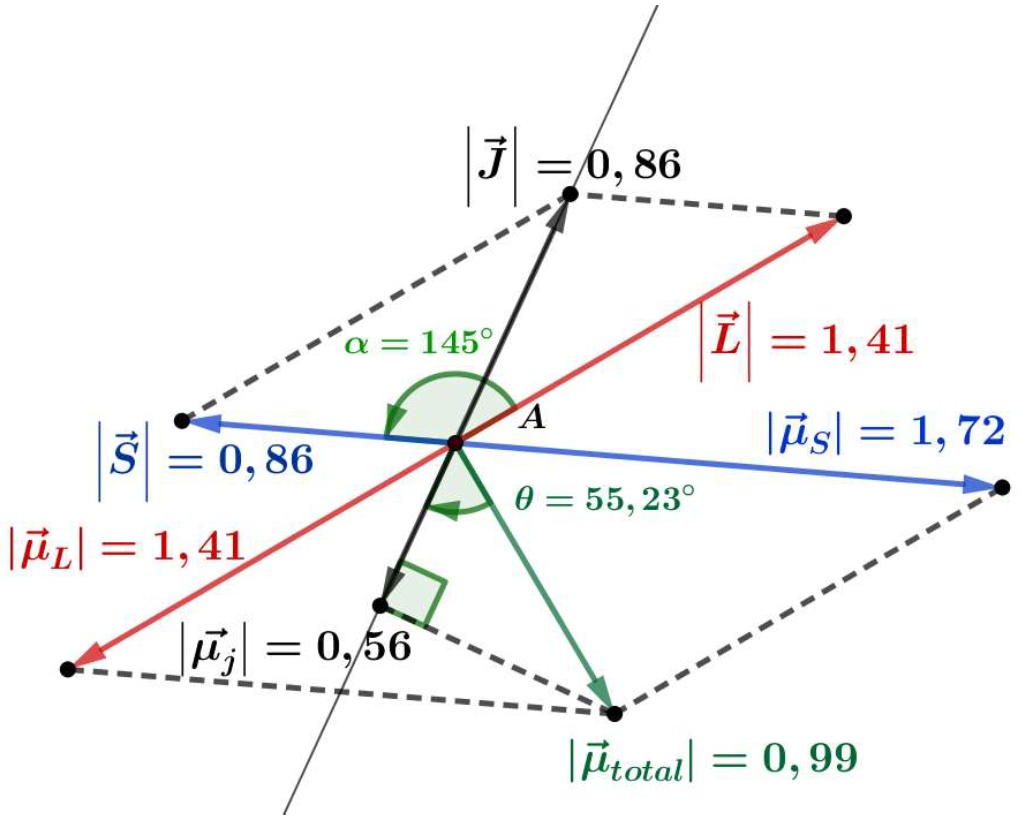
\includegraphics[width=0.8\textwidth]{./Figures/fig_s1}
	\caption{Cálculo geométrico de $\mu_{j}$ }
	\label{fig:s1}
\end{figure}

\subsection{Propiedades magnéticas:}


\begin{figure}[H]
    \centering
    \textbf{Observar los orbitales incompletos}
    \vspace{1.0cm}
    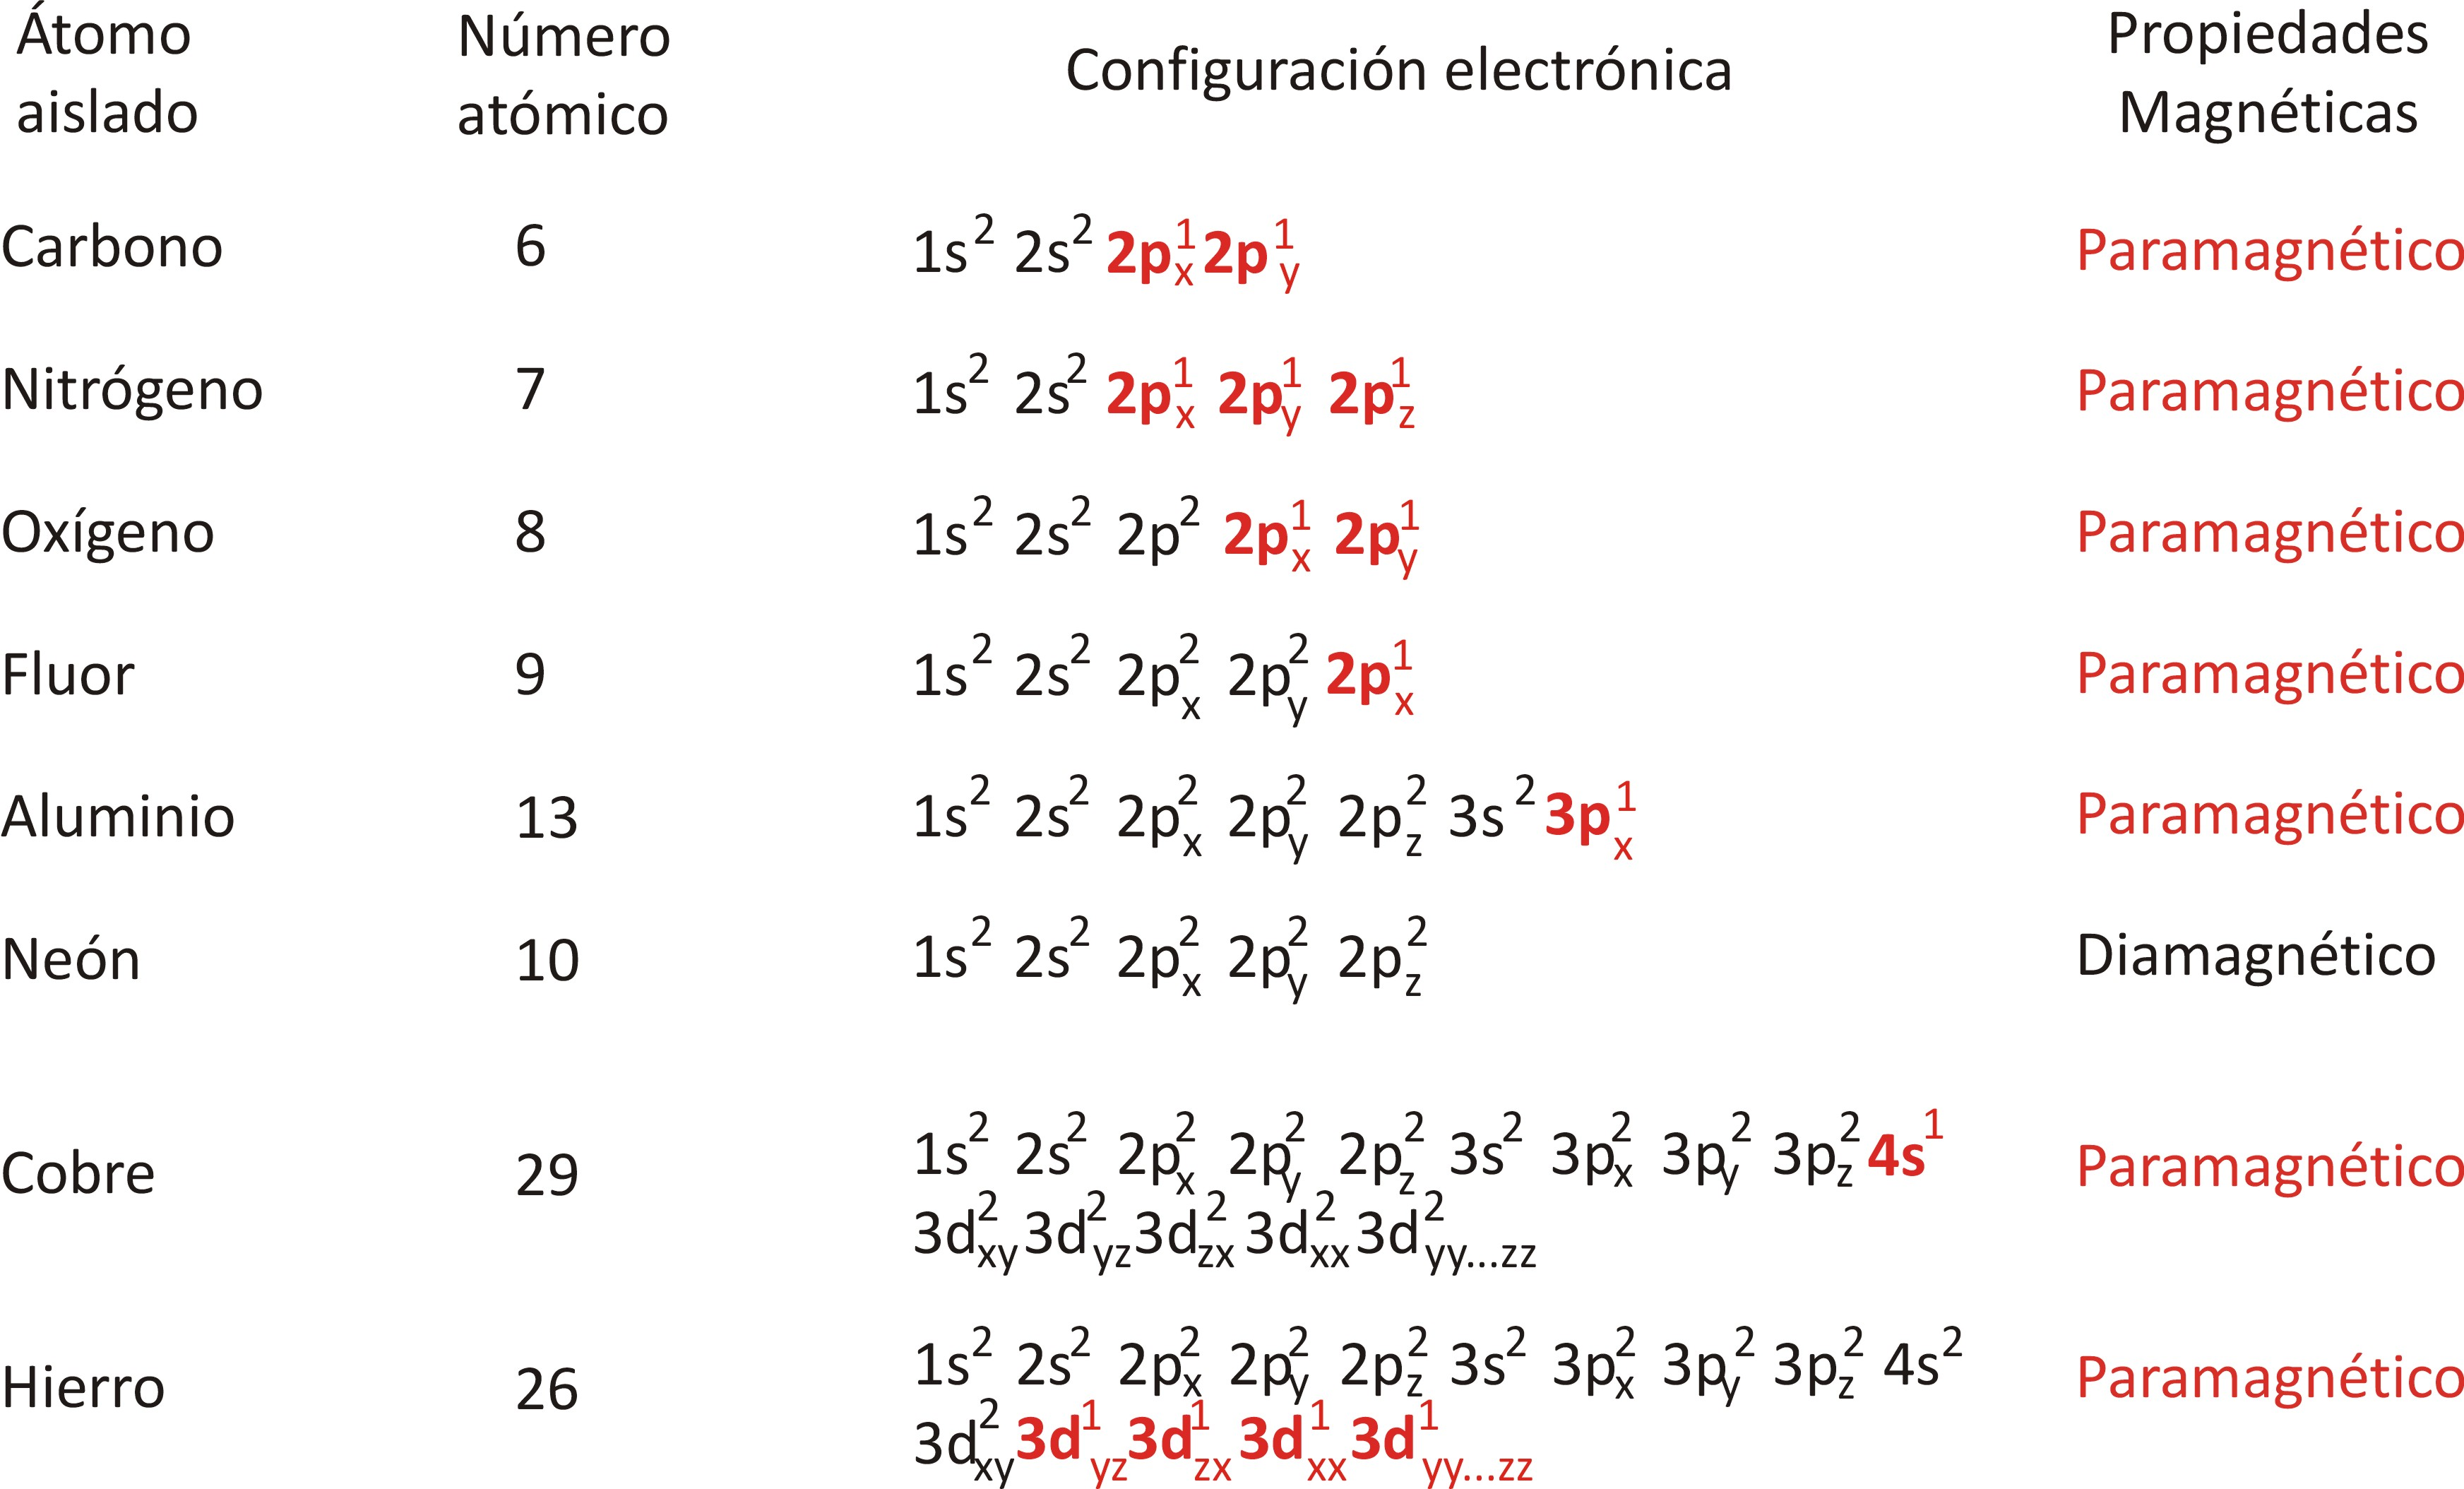
\includegraphics[width=1.0\textwidth]{./Figures/PropMagneticasDeAlgunosAtomos}
	\caption{Propiedades magnéticas de algunos átomos}
	\label{fig:PropMagneticasDeAlgunosAtomos}
\end{figure}


\subsection{Paramagnetismo en átomos con varios electrones}

Las propiedades magnéticas de los átomos se determina, entre otros, por el momento angular total del mismo Si el átomo esta aislado el momento angular total es constante Para hallar el momento magnético de un átomo con más de un electrones, suponiendo interacción de Russell Saunders, se debe tener en cuenta los espines de los electrones de las capas no completa y sus momentos angulares. Como se vio anteriormente, para encontrar debemos hacer

\begin{equation}
\V{S}=\sum_{i}\V{s_{i}} \quad, \quad \V{L}=\sum_{i}\V{l_{i}} 
\end{equation}

Donde la suma se extiende a cada uno de los electrones. Normalmente la nomenclatura utilizada en este tema, indica las características cuánticas del átomo con varios electrones y son las mismas anteriores pero en letras mayúsculas:

\begin{equation}
	|\V{L}|=\sqrt{L\big(L+1\big)}\,\hbar \;,\; |\V{S}|=\sqrt{L\big(S+1\big)}\,\hbar \;,\; |\V{J}|=\sqrt{J\big(J+1\big)}\,\hbar
\end{equation}

Mientras que las componentes en la dirección $z$ son:

\begin{equation}
	L_{z}=M_{L}\hbar \quad, \quad S_{z}=M_{S}\hbar  \quad, \quad J_{z}=M_{J}\hbar 
\end{equation}

Los números cuánticos del átomo están relacionados con los números cuánticos de los electrones individuales:

\begin{equation}
M_{L}=\sum_{i}\big( m_{li}\big)_{z} \;,\; M_{S}=\sum_{i}\big( m_{si}\big)_{z} \;,\;M_{J}=M_{L}+M_{S}
\end{equation}

Conociendo $M_{L}$, $M_{S}$, $M_{J}$ se puede deducir $L$, $S$, $J$:

\begin{equation}
\begin{aligned}
	M_{L} &= \lbrace L, \big(L-1\big), \big(L-2\big),..., -L\rbrace \\
	M_{S} &= \lbrace S, \big(S-1\big), \big(S-2\big),..., -S\rbrace \\
	M_{J} &= \lbrace J, \big(J-1\big), \big(J-2\big),..., -J\rbrace 
\end{aligned}
\end{equation}


La notación electrónica es usada generalmente para describir el estado fundamenta del átomo. Pero cuando están excitados esta notación no es adecuado y se usa la notación espectroscópica. Esta notación se caracteriza por que cada estado posible del átomo en su totalidad se encuentra representado por los números cuánticos $L$, $S$, $J$ (mayúscula no confundir). El valor particular de $L$ para un determinado estado atómico se designa mediante letras mayúsculas:

\begin{figure}[H]
    \centering
    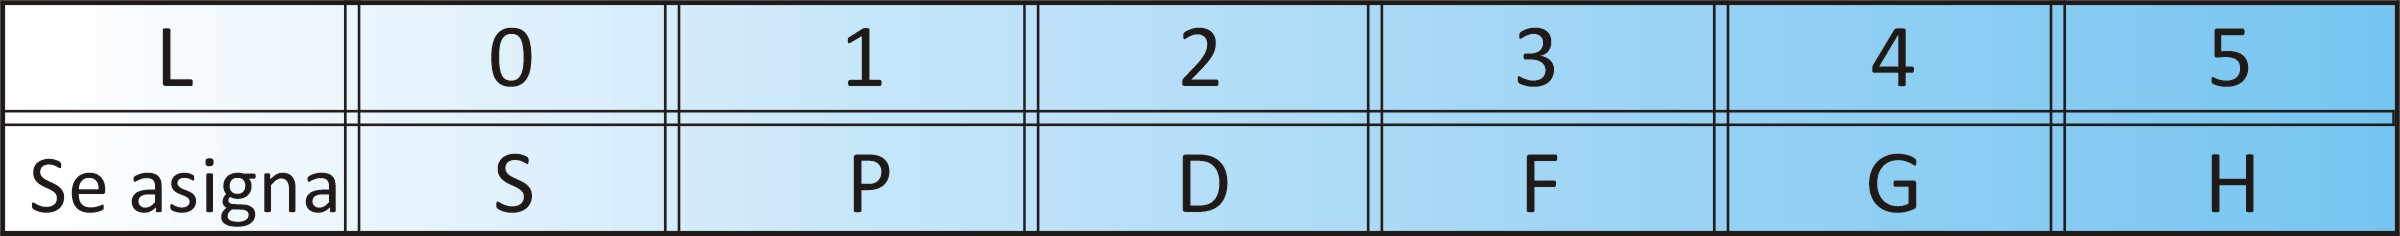
\includegraphics[width=0.8\textwidth]{./Figures/LSeAsigna}
	\caption{Notación espectroscópica}
	\label{fig:LSeAsigna}
\end{figure}

Luego se trabaja con la notación espectroscópica o de Russell que se indica según:

\begin{figure}[H]
    \centering
    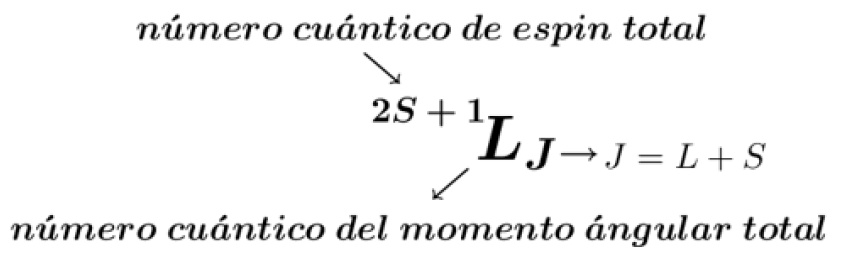
\includegraphics[width=0.6\textwidth]{./Figures/NotacionEspectroscopica}
	\caption{Notación de Rusell}
	\label{fig:NotacionEspectroscopica}
\end{figure}

\begin{itemize}
\item Vimos que el estado de un átomo se conoce cuando sabemos cuantos electrones y con que espín ocupan cada orbital ($n$, $l$, $m_{l}$).

\item La energía $\varepsilon_{nl}$ de cada sistema espín orbita depende solo de $n$ y $l$ entonces, como existenexisten $2l+1$ orbitales con la misma energía y como cada orbital puede tener como máximo dos electrones apareados, el número de estados para una dada energía es ($2l+1$) y es el grado de degeneración.

\item \textbf{Ejemplo} el hidrogeno tiene la siguiente configuración electrónica $1s^{1}$ ,luego $n=1$, $l=0$, $m_{l}=0$ y $m_{s}=\pm \frac{1}{2}$ los dos estados tienen igual energía y la degeneración es $2(2l+1)=2$.

\item También se sabe que la energía de un estado (en el caso de un átomo con varios electrones) no depende de $M_{L}$ ni de $M_{S}$ Luego la degeneración de cada estado es el producto de los posibles valores de $M_{L}$ y $M_{S}$ para un dado $L$ y $S$.
\begin{equation}
	(2L+1)(2S+1)
\end{equation}

\item Se debe aclarar que existe otra forma (aparte de la de Russell Saunders) de sumar los momento angulares La forma alternativa de acoplamiento, espín órbita, cuando el espín y los momentos angulares orbitales dependen fuertemente unos de otros se llama acoplamiento $j-j$ Esta forma de acoplamiento es aplicable a átomos muy pesados. Aqui se  asume que hay una fuerte interacción $s-l$ y que este acoplamiento es más fuerte que el $l-l$ Como los vectores fuertemente acoplados se suman primero, estos dan una $j$ resultante para cada electrón. Los $j$ vectores se suman para obtener $J$ para todo el átomo.
\end{itemize}

Observemos que para una configuración dada pueden existir varios valores de $L$,dependiendo de la orientación relativa de los vectores, de igual manera para el espín, dada una configuración pueden corresponder varios valores de $S$. El estado de un átomo esta determinado por los números cuánticos $L$, $S$ y $J$. A los estados de una configuración con igual $S$, $L$ se lo llaman terminales. Seguidamente veremos ejemplos del calculo y notación, por lo general es un conjunto de reglas empíricas

1.- Se determinan las sumas:
\begin{equation}
M_{L}=\sum_{i}\big( m_{li}\big)_{z} \;,\; M_{S}=\sum_{i}\big( m_{si}\big)_{z} 
\end{equation}

2.-éstas nos proporcionan los posibles valores de $M_{L}$ y $M_{S}$, luego se puede inferir de ellos los posibles valores de $S$ y $L$.

Veamos el caso de una \textbf{configuración completa con subcapas cerradas}. Los electrones apareados tienen $m_{s}=+\dfrac{1}{2}$ y $m_{s}=-\dfrac{1}{2}$, luego $M_{S}=\sum_{i}\big( m_{si}\big)_{z}=0$ algo similar sucede con el impulso angular, hay iguales proyecciones hacia arriba como hacia abajo luego, $M_{L}=\sum_{i}\big( m_{li}\big)_{z}=0$ para configuraciones completa $p^{6}$, $d^{10}$ y $f^{14}$ es siempre cero, por ejemplo, si tomamos el orbital $p^{6}$ le corresponde $l=1$ luego $m_{l}=1,0,-1$ para cada electrón y tenemos seis de ellos.

Para $p^{6}$ cada electrón tendrá un $m_{l}$ entre los siguientes valores $1,0,−1$

\begin{equation*}
\begin{aligned}
	M_{L} &= m_{l1}+m_{l2}+m_{l3}+m_{l4}+m_{l5}+m_{l6}=1+1+0+0+-1-1=0\\
	M_{S} &= m_{s1}+m_{s2}+m_{s3}+m_{s4}+m_{s5}+m_{s6}=\dfrac{1}{2}-\dfrac{1}{2}+\dfrac{1}{2}-\dfrac{1}{2}+\dfrac{1}{2}-\dfrac{1}{2}=0
\end{aligned}
\end{equation*}

Los únicos posibles valores de $S$ y $L$ son cero Las subcapas cerradas pueden ignorarse ya que no contribuyen.

Si varios electrones se encuentran en orbitales distintas decimos que no son equivalentes, ya que no hay restricciones por el principio de Pauli y pueden tomar distintas combinaciones de $m_{l}$ y $m_{s}$.

\textbf{Subcapa abierta con electrones equivalentes} supongamos una configuración electrónica $p^{1}$ y $d^{1}$ luego $l_{1}=1$ y $l_{2}=2$. Los valores de $L$ y $S$ se determinan de:

\begin{equation*}
	(l_{1}+l_{2}, l_{1}+l_{2}-1, l_{1}+l_{2}-2, \cdots, |l_{1}-l_{2}|)= L= (3, 2, 1)
\end{equation*}
Los
posibles valores de $S$ son:
\begin{equation*}
	(s_{1}+s_{2}, s_{1}+s_{2}-1, s_{1}+s_{2}-2, \cdots, |s_{1}-s_{2}|)= L= (1, 0)
\end{equation*}

Por tanto todos los casos posibles son:

\begin{equation*}
\begin{aligned}
	&L=1 \text{y} S=1 \Rightarrow (2L+1)(2S+1)=9\;\Rightarrow J=L+S=2\Rightarrow {^{3}}P_{2}\\
	&L=1 \text{y} S=0 \Rightarrow (2L+1)(2S+1)=3\;\Rightarrow J=L+S=1\Rightarrow {^{1}}P_{1}\\			&L=2 \text{y} S=1 \Rightarrow (2L+1)(2S+1)=15\Rightarrow J=L+S=3\Rightarrow {^{3}}P_{3}\\
	&L=2 \text{y} S=0 \Rightarrow (2L+1)(2S+1)=5\;\Rightarrow J=L+S=2\Rightarrow {^{1}}P_{2}\\
	&L=3 \text{y} S=1 \Rightarrow (2L+1)(2S+1)=21\Rightarrow J=L+S=4\Rightarrow {^{3}}P_{4}\\
	&L=3 \text{y} S=0 \Rightarrow (2L+1)(2S+1)=7\;\Rightarrow J=L+S=4\Rightarrow {^{1}}P_{3}
\end{aligned}
\end{equation*}


\begin{equation*}
	(L+S, L+S-1, L+S-2, \cdots, |L-S|)= J = (4, 3, 2, 1)
\end{equation*}

\textbf{Subcapa abierta con electrones no equivalentes}, o sea con varios electrones en una misma subcapa En este caso debemos tener en cuenta las restricciones impuestas por el principio de Pauli Generalmente para conocer cual es el estado fundamental o de mínima energía de todos los posibles estados energéticos de una configuración electrónica se lo encuentra directamente aplicando las reglas de Hund.

Cuando vimos como se llenaban los orbitales de un átomo con los electrones para dar origen a los distintos elementos de la tabla periódica, mencionamos las reglas de Hund Estás, pueden ser usadas también, para calcular $L$,$S$ y $J$. Si son aplicadas a los electrones en una capa para determinar el estado del átomo Las reglas son tres y se aplican el espín, al momento angular orbital y al momento angular atómico.

\begin{itemize}
\item[1] El estado de mínima energía es el que tiene mayor multiplicidad de espín, de otro modo, los electrones orientan sus espines paralelamente en capas incompletas y el máximo momento angular del átomo debido al espín es $S=\sum m_{s}$.


\item[2] Si hay más de un termino, para una configuración dada, con la máxima multiplicidad, el de menor energía es el de mayor valor de $L$ O bien, el máximo valor del momento angular orbital atómico se lo obtiene de $L=\sum m_{l}$.


\item[3] Si la configuración electrónica esta menos de la mitad ocupada, el estado mas estable es el $J=L-S$ por el contrario, si esta mas de la mitad ocupado el estado fundamentales $J=L+S$
\end{itemize}

Veamos distintos ejemplos:

El ion $S_{m}^{3+}$ tiene 5 electrones en la capa $4f$ encontrar $S$, $L$ y $J$.

La capa $f$ corresponde a $l=3$ luego se encuentran los posibles $m_{l}$ y $m_{s}$ para
posteriormente llenarlos con los electrones de acuerdo con las reglas de Hund.


\begin{figure}[H]
    \centering
    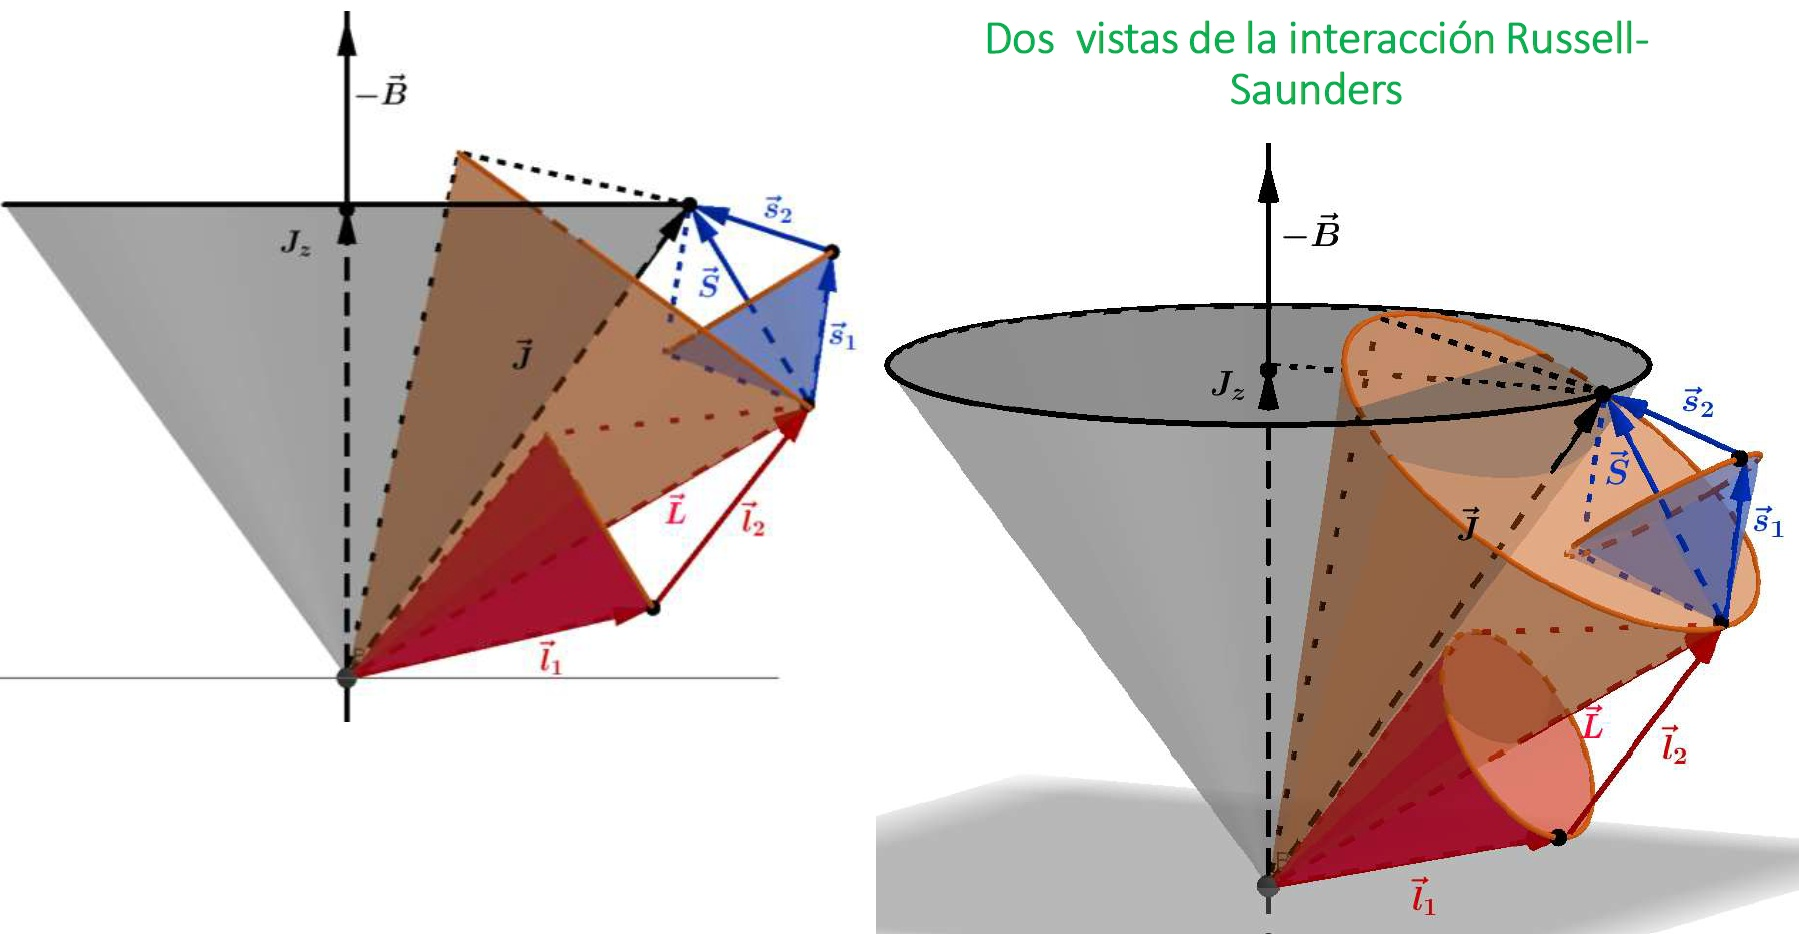
\includegraphics[width=1.0\textwidth]{./Figures/fig_s2}
	\caption{Interacción de Rusell-Saunders}
	\label{fig:s2}
\end{figure}

Vemos en la figura \ref{fig:s3} que sumamos los $m_{l}$ y $m_{s}$ en los lugares donde hay aporte de electrones y como la capacidad de $f$ es 14 entonces, $J=L-S=\dfrac{5}{2}$. Vemos que con este procedimiento no es necesario encontrar todos los casos posibles como se hizo en ejemplos anteriores. Desde el punto de vista del magnetismo solo nos interesa conocer el $J$. Observemos también que debemos conocer como se ioniza el átomo en estudio

\begin{figure}[H]
    \centering
    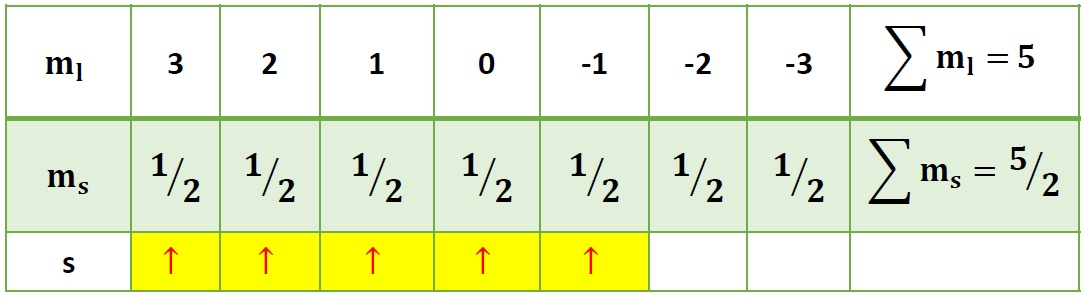
\includegraphics[width=0.8\textwidth]{./Figures/fig_s3}
	\caption{Momentos en el átomo}
	\label{fig:s3}
\end{figure}

El ion $Fe^{2+}$ con 6 electrones en $3d$, lo cual implica que $l=2$, la capacidad de $d$ es 10,luego observemos la distribución de momentos en la figura \ref{fig:s4}:

\begin{figure}[H]
    \centering
    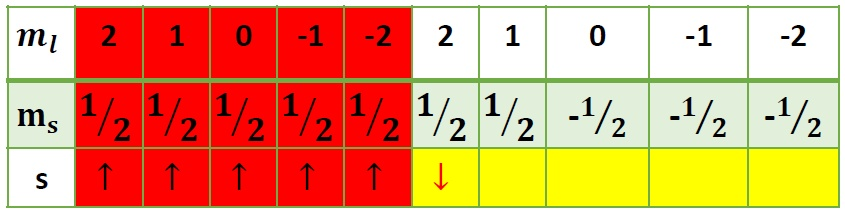
\includegraphics[width=0.8\textwidth]{./Figures/fig_s4}
	\caption{Momentos del $Fe^{2+}$}
	\label{fig:s4}
\end{figure}

$\sum m_{l}=2$ y $\sum n_{s}=2$ y la capacidad de $ds$ es de 10, tiene mas de la mitad ocupada, luego $2S+1=5$, $J=L+S=4$, por tanto la notación espectral es $^{5}D_{4}$

Otro ejemplo: Escriba en la notación espectral el termino de mas baja energía para la configuración $d^{3}$ de acuerdo a las reglas de Hund. vemoa la figura \ref{fig:s5}

$\centerdot$ $l=2$, por Pauli y la primera regla de Hund, tenemos:

\begin{figure}[H]
    \centering
    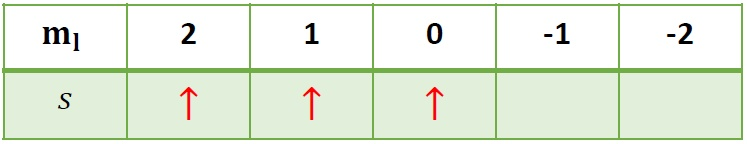
\includegraphics[width=0.8\textwidth]{./Figures/fig_s5}
	\caption{Configuración $d^{3}$}
	\label{fig:s5}
\end{figure}

El término de más baja energía tendrá $S=\dfrac{3}{2}\rightarrow 2S+1=4$

$\centerdot$ El valor máximo de $L$ es 3 $\rightarrow F$

%$\centerdot$ $J$ sera $J=L-S=3-\dfrac{3}{2}=\dfrac{3{2}\rightarrow ^{4}F_{\frac{3}{2}}$ menos de la mitad ocupadas. 

Otro ejemplo, en la figura \ref{fig:s6} vemos el cálculo para otro elemento perteneciente a la serie de los Lantánidos $4f3$:

$\centerdot$ $l=3$

\begin{figure}[H]
    \centering
    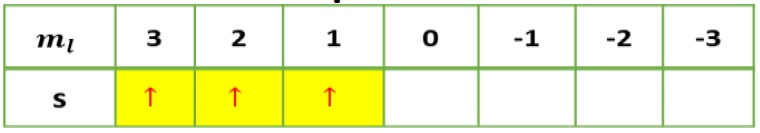
\includegraphics[width=0.8\textwidth]{./Figures/fig_s6}
	\caption{Configuración $4f^{3}$}
	\label{fig:s6}
\end{figure}

$S=\dfrac{3}{2}\rightarrow 2S+1=4$, el valor máximo de $L=6 \rightarrow I$ y $J=L-S=\dfrac{9}{2}\rightarrow {^{3}}I_{\frac{9}{2}}$

Ejercicio: calcular el momento magnético de $F3^{2+}$.

Como se vio la estructura electrónica del hierro es $Fe = [Ar]3d^{6}4s^{2} \rightarrow Fe^{2+}=[Ar]3d^{6}4s^{0}$, luego como vimos en el ejercicio anterior quedan cuatro electrones sin aparear, lo cual nos dio $L=4$ y $S=2$ con $J=4$

\begin{equation*}
	g_{j}= 1 +\dfrac{\qa{l}+\qa{s}-\qa{l}}{2\qa{j}}=1+\dfrac{20}{40}=1,5
\end{equation*}

\begin{equation*}
	\mu_{j}= g_{j}\sqrt{\qa{j}}\mu_{B}=1,5\sqrt{20}\mu_{B}=6,70\mu_{B}
\end{equation*}


El valor experimental es $5,4 \mu_{B}$. Si calculamos solo la contribución del espín, sabiendo que $g_{s}\approx 2$

\begin{equation*}
	s= g_{j}\sqrt{\qa{Sj}}\mu_{B}=2\sqrt{6}\mu_{B}=4,89\mu_{B}
\end{equation*}


Vemos que se aproxima más a los datos experimentales si solo trabajamos con el espín, esto significa que el impulso angular no participa $S$ sucede lo mismo en toda la serie $3d$, como fue comentado anteriormente, luego, el momento magnético esta solo determinado por el espín.


\section{Paramagnetismo (enlace iónico)}

$\centerdot$ En general hemos hablado, hasta ahora, de momentos magnéticos de átomos aislados, sabiendo que la gran mayoría de los átomos tienen momento magnético diferente de cero Pero la generalidad de los cuerpos están formados por moléculas y esto cambia la cosa, resultando mayor el número de sustancias solamente diamagnéticas, por el contrario las moléculas paramagnéticas escasean. Veamos un caso que al combinarse átomos paramagnéticos para formar un sólido este resulta no ser paramagnético:

La configuración electrónica del sodio y el cloro son:

\begin{equation*}
\begin{aligned}
	Na:\; &1s^{2}2s^{2}2p^{6}3s^{1}=[Ne]3S^{1}\\
	Cl:\; &1s^{2}2s^{2}2p^{6}3s^{2}39^{5}=[Ne]3S^{2}3p^{5} 
\end{aligned}
\end{equation*}

vemos que al sodio le sobra un electrón para tener una estructura mas estable y al cloro le faltaría uno para ser más estable. También vemos que ambos son paramagnéticos. Luego cuando se forma el $ClNa$ se crea el ion $Na^{+}$ pareciéndose al $Ne$ y el ion $Cl^{-}$ con electrónica análoga al $Ar$, por tanto debido a esta unión el compuesto $ClNa$ no es paramagnético

\subsection{Paramagnetismo en un sólido}


\begin{itemize}
	\item El \textbf{paramagnetismo} en un sólido es la tendencia de los momentos magnéticos atómicos (espín u orbital) a alinearse paralelamente a un campo magnético externo.
	
	\item Se produce por la alineación individual de los momentos magnéticos de los átomos o moléculas bajo la presencia de un campo magnético externo. Esto puede ser en átomos individuales o en sólidos.
	
	\item Debido a la agitación térmica, cuando sacamos el campo magnético externo desaparece el paramagnetismo.
	
	\item Puesto que la agitación distribuye aleatoriamente la dirección de los dipolos magnéticos, un aumento de la temperatura disminuye el efecto paramagnético.
	
	\item En el paramagnetismo $\chi>0$, $|\chi|\approx 10^{-4}$ a temperatura ambiente, es función de T:

	\begin{equation}
  		\V{M}=\chi\V{B}=\frac{C}{T-\vartheta}\V{B} \quad \text{Ecuación de Curie-Weiss}
	\end{equation}

	Con $C$ y $\vartheta$ constantes. A bajas temperaturas los sistemas se apartan de este comportamiento. Esta ley deja cumplirse cuando se aproxima a la saturación, o sea que la mayoría de los momentos magnéticos están alineados.
\end{itemize}


\subsection{Paramagnetismo clásico}

Si bien el magnetismo es un fenómeno netamente cuántico, algunas mecanismos pueden ser visualizados clásicamente, siempre y cuando den resultados equivalentes.

Consideremos la figura \ref{fig:s7}, tenemos el átomo como un núcleo central y los electrones orbitando (clásicamente) alrededor de él. Cada órbita puede asimilarse a una corriente eléctrica Bajo la suposición anterior calculemos el momento magnético orbital de un electrón en una orbital circular. Si $v=\frac{\omega}{2\pi}$ es la frecuencia del movimiento, la corriente será $i=ev$, luego el momento magnético es

\begin{figure}[H]
    \centering
    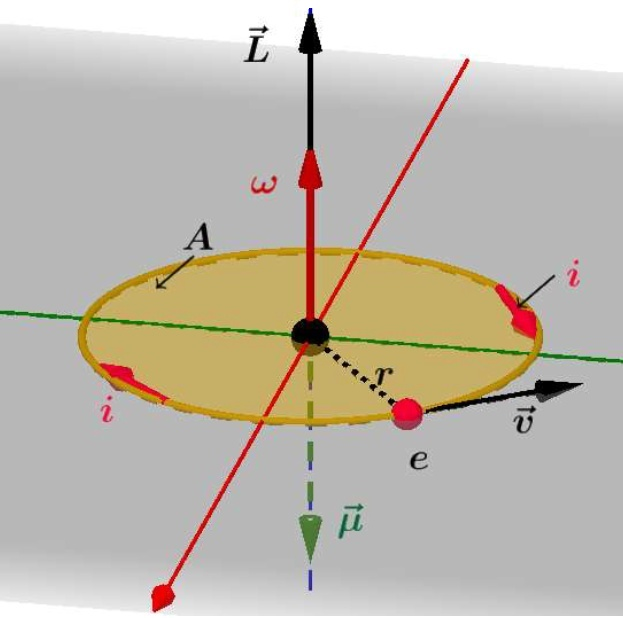
\includegraphics[width=0.7\textwidth]{./Figures/fig_s7}
	\caption{Representación clásica del paramagnetismo}
	\label{fig:s7}
\end{figure}


\begin{equation}
  \mu= iA = e \frac{\omega}{2\pi}A = e \frac{\omega}{2\pi} \pi r^{2}
\end{equation}

Donde $A$ es el área y $\mu$ es opuesto al momento angular orbital $L$. Si $m$ es la masa del electrón el momento angular orbital $L$ sera:

\begin{equation}
  L=mvr=m\omega r^{2}
\end{equation}


\begin{equation}
  \mu=\frac{e\omega r^{2}}{2}=\frac{e}{2m}L
\end{equation}

Similar al cuántico definido anteriormente, solo faltaría el signo menos que indica sentidos opuestos.

Por otro lado sabemos que la energía $\Bb{\varepsilon}_{M}$ del momento magnético $\V{\mu}$ en un campo magnético $\V{B}$ es 

\begin{equation*}
	\Bb{\varepsilon}_{M}=-\V{\mu}\cdot \V{B}= |\V{\mu}||\V{B}|Cos(\vartheta)
\end{equation*}

Esta claro que si el ángulo $\vartheta$ entre \V{\mu} y \V{B} es $0^{o}$ o $180^{o}$ la
energía es mínima.

Previamente recordemos dos ideas fundamentales de la mecánica clásica, con el objeto de entendamos correctamente el tema que desarrollaremos La primera indica que la variación de la cantidad de movimiento lineal es igual a la suma de la fuerzas externas que actúan sobre el cuerpo $\dTv{P}{t}=\V{f}_{ext}$. Mientras que la segunda, es su equivalente en el movimiento angular, el cambio en el vector cantidad de movimiento angular es igual a la suma de los momentos de las fuerzas externas  $\dTv{L}{t}=\V{M}_{ext}$

Es oportuno recordar el movimiento de un trompo, se sabe que si el cuerpo gira a una velocidad $\omega$ sobre su eje de simetría y esta en presencia de una cupla externa, en este caso la gravedad Se agrega un nuevo movimiento llamado precesión, debido a la interacción con la fuerza gravitatoria Algo similar sucede con nuestro electrón cuando agregamos un campo magnético externo Se genera la precesión de Larmor Este termino hace referencia a la precesión de los momentos magnéticos de electrones o núcleos, por la acción de un campo magnético $\V{B}$ externo pequeño, constante y homogéneo.

\begin{equation*}
	\dTv{L}{t}=\V{M}_{ext} = \V{\mu} \times \V{B} = -\dfrac{e}{2m}\V{L}\times\V{B}\rightarrow |\dTv{L}{t}|= |\V{\mu}||\V{B}| Sin(\alpha)
\end{equation*}

Como tenemos una cupla externa distinta de cero |\V{L}| no es constante, pero si es constante el modulo de $\V{L}$.

Suponngamos $\omega$ es la velocidad angular del electrón. Como el movimiento es circular debe existir una aceleración centrípeta responsable del cambio de la velocidad. La fuerza sobre el electrón debido al núcleo será, como vemos en la figura \ref{fig:s8}:

\begin{figure}[H]
    \centering
    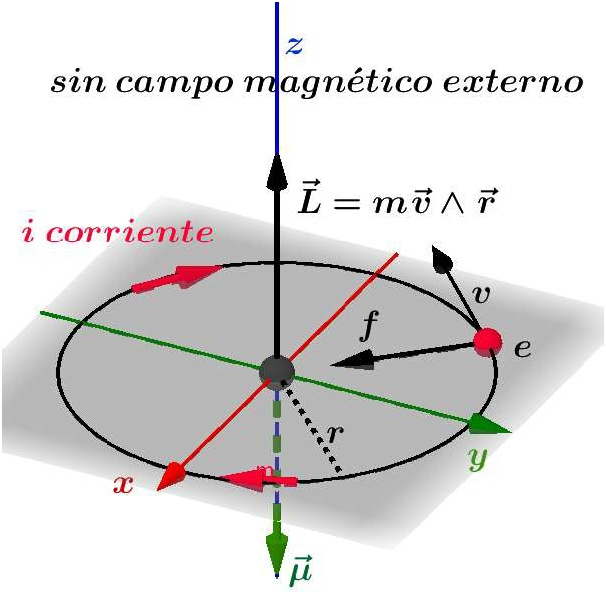
\includegraphics[width=0.7\textwidth]{./Figures/fig_s8}
	\caption{Sin campo exterior}
	\label{fig:s8}
\end{figure}

\begin{equation}
  f=ma_{cp}=m\omega^{2} r
\end{equation}

Si se aplica un campo magnético $\V{H}$ perpendicular al plano de rotación como se observa en la figura \ref{fig:s9}, sabemos se ejerce sobre el electrón una nueva fuerza que de acuerdo con la ecuación de Lorentz:

\begin{equation}
  \V{f}_{l}= e\V{E} + ev \times \V{H} = ev \times \V{H}
\end{equation}

\begin{figure}[H]
    \centering
    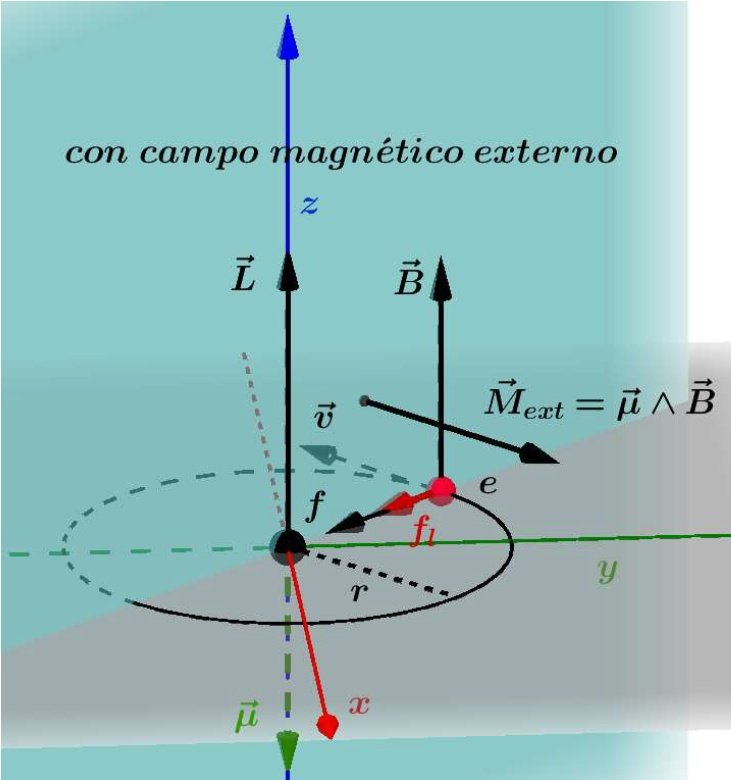
\includegraphics[width=0.7\textwidth]{./Figures/fig_s9}
	\caption{Campo exterior perpendicular}
	\label{fig:s9}
\end{figure}



Ya que campo eléctrico no hay, tenemos solo la fuerza magnética, que es también radial, luego:

\begin{equation}
  f+f_{l}= m\omega^{2}r+ evH = m\omega^{2}r+ e\omega_{1}rH=m\omega_{1}^{2}r
\end{equation}

\begin{equation}
  \omega_{1}^{2}-\frac{eH}{m}\omega_{1}-\omega^{2} =0
\end{equation}

\begin{equation}
	\omega_{1}=\frac{\frac{eH}{m}\sqrt{\big(\frac{eH}{m}\big)^{2}+4\omega^{2}}}{2}
\end{equation}

Se demuestra que $\big(\frac{eH}{m}\big)^{2}\ll 4\omega^{2}$ luego

\begin{equation}
	\omega_{1}= \omega^pm\frac{eH}{2m}\Delta\omega=\pm\frac{eH}{2m}
\end{equation}

Llamada frecuencia de Larmor. \textbf{El campo magnético aplicado hace variar la velocidad angular del electrón. En la expresión no figura el radio de la órbita ni la velocidad de rotación del electrón luego $\Delta\omega$ es la misma para cualquier órbita}. El campo $\V{B}$ es el responsable del movimiento de precesión de $\V{L}$ alrededor de $\V{B}$ similar al trompo con la gravedad.

\begin{figure}[H]
    \centering
    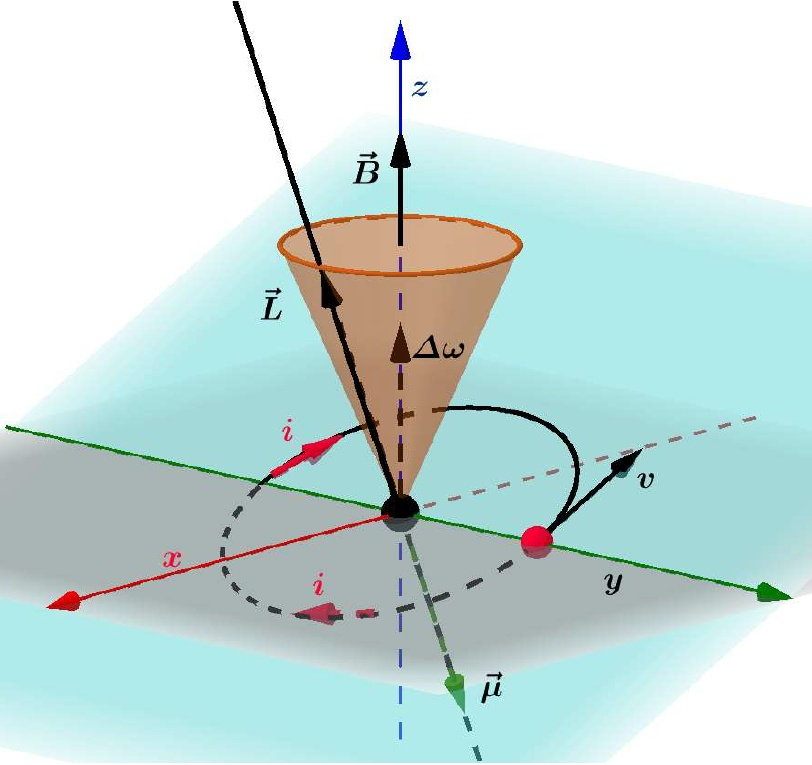
\includegraphics[width=0.7\textwidth]{./Figures/fig_s10}
	\caption{Precesión de $L$ alrededor de $B$}
	\label{fig:s10}
\end{figure}

\textbf{Resumiendo lo encontrado}:

La velocidad del electrón en su órbita es $\omega$ La velocidad de rotación (precesión) de $L$ alrededor de $B$ es la frecuencia de Larmor $\Delta\omega=\pm\frac{eH}{2m}$ que es también la
frecuencia de rotación del plano orbital El campo magnético hace variar la velocidad angular del electrón proporcional al campo. Observamos que no figura en $\Delta\omega$, el radio de la orbita ni la velocidad del electrón, por tanto, es la misma frecuencia para cualquier órbita.
Podemos afirmar que el electrón con la introducción del campo tiene un nuevo movimiento circular adicional alrededor del campo,campo,(o bien un cambio en su velocidad angular) como vemos en la
figura Esto generara un nuevo momento magnético responsable del diamagnetismo, como veremos más
adelante.




















\subsubsection{Teorema de Larmor}
En mecánica elemental estudiamos el movimiento de un trompo, vimos que si el cuerpo gira a una velocidad $\omega$ sobre su eje de simetría y esta en presencia de una fuerza externa, gravedad. Se agrega un nuevo movimiento llamado precesión, debido a la interacción con la fuerza gravitatoria.

\begin{figure}[H]
    \centering
    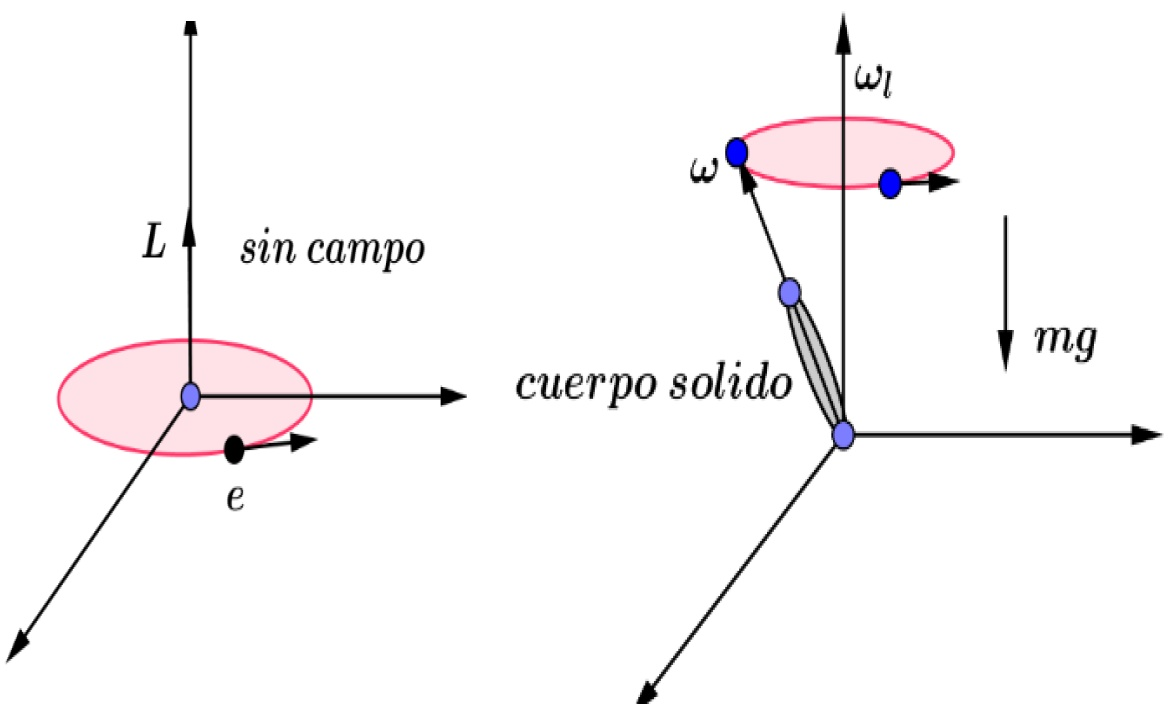
\includegraphics[width=0.8\textwidth]{./Figures/Larmor1}
	\caption{Precesión de un trompo en el campo gravitatorio}
	\label{fig:Larmor1}
\end{figure}

Este teorema afirma que si tenemos una partícula cargada orbitando en un campo de fuerzas centrales y le aplicamos un pequeño campo magnético, este produce un movimiento adicional de precesión que se superpone al movimiento original. Dicho de otro modo el movimiento original es el mismo solo se agrega una precesión del momento magnético alrededor del vector campo magnético (en primer orden de $\overrightarrow{H}$) con frecuencia $\omega_{l}$ de Larmor

\begin{figure}[H]
    \centering
    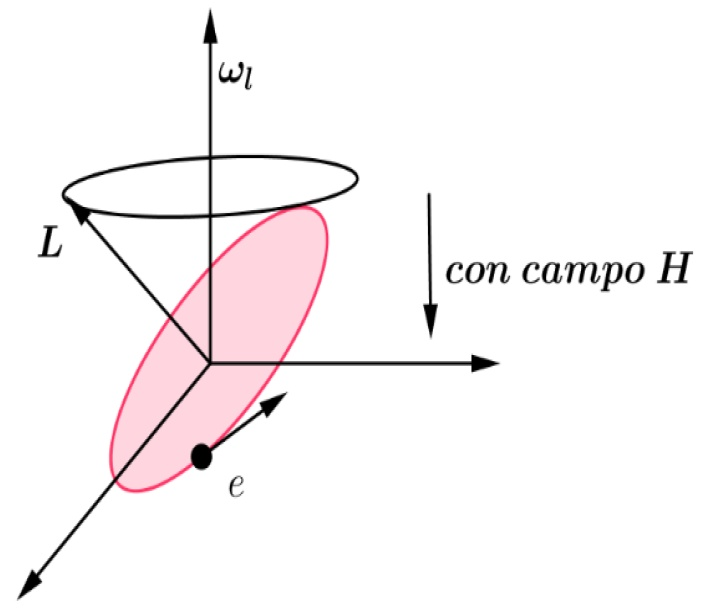
\includegraphics[width=0.6\textwidth]{./Figures/Larmor2}
	\caption{Precesión de Larmor debido al campo H}
	\label{fig:Larmor2}
\end{figure}


Si la órbita no es perpendicular al campo o sea que forma un ángulo determinado entonces precede alrededor del campo magnético describiendo un cono alrededor de $\overrightarrow{H}$. En consecuencia surge un momento magnético adicional que se opone al cambio de velocidad angular

\begin{equation}
  \mu= -iA = -e \frac{\Delta\omega}{2\pi}A = -\frac{e^{2}A}{4\pi m} H
\end{equation}

Si el átomo tiene $z$ electrones

\begin{equation}
  \mu= -\frac{z e^{2}A}{4\pi m} H = -\frac{z e^{2} \overline{r^{2}}}{4m} H
\end{equation}

Donde $\overline{r^{2}}$ es el cuadrado medio de la distribución de probabilidad del electrón. Si $N$ es el número de átomos por unidad de volumen tendremos que la susceptibilidad magnética por unidad de volumen será:

\begin{equation}
  \chi= -\frac{z N e^{2}}{4m} \overline{r^{2}}
\end{equation}

Vemos que el problema de calcular la susceptibilidad diamagnética reside en calcular $\overline{r^{2}}$ o sea, la distribución de carga electrónica. Se destaca también que la susceptibilidad diamagnética no depende de la temperatura y crece con el número atómico del elemento.

En este calculo semiclásico se supuso que todos los electrones están ligados a los átomos, cosa que es cierta en los dieléctricos mas no en los metales o semiconductores.

\begin{figure}[H]
    \centering
    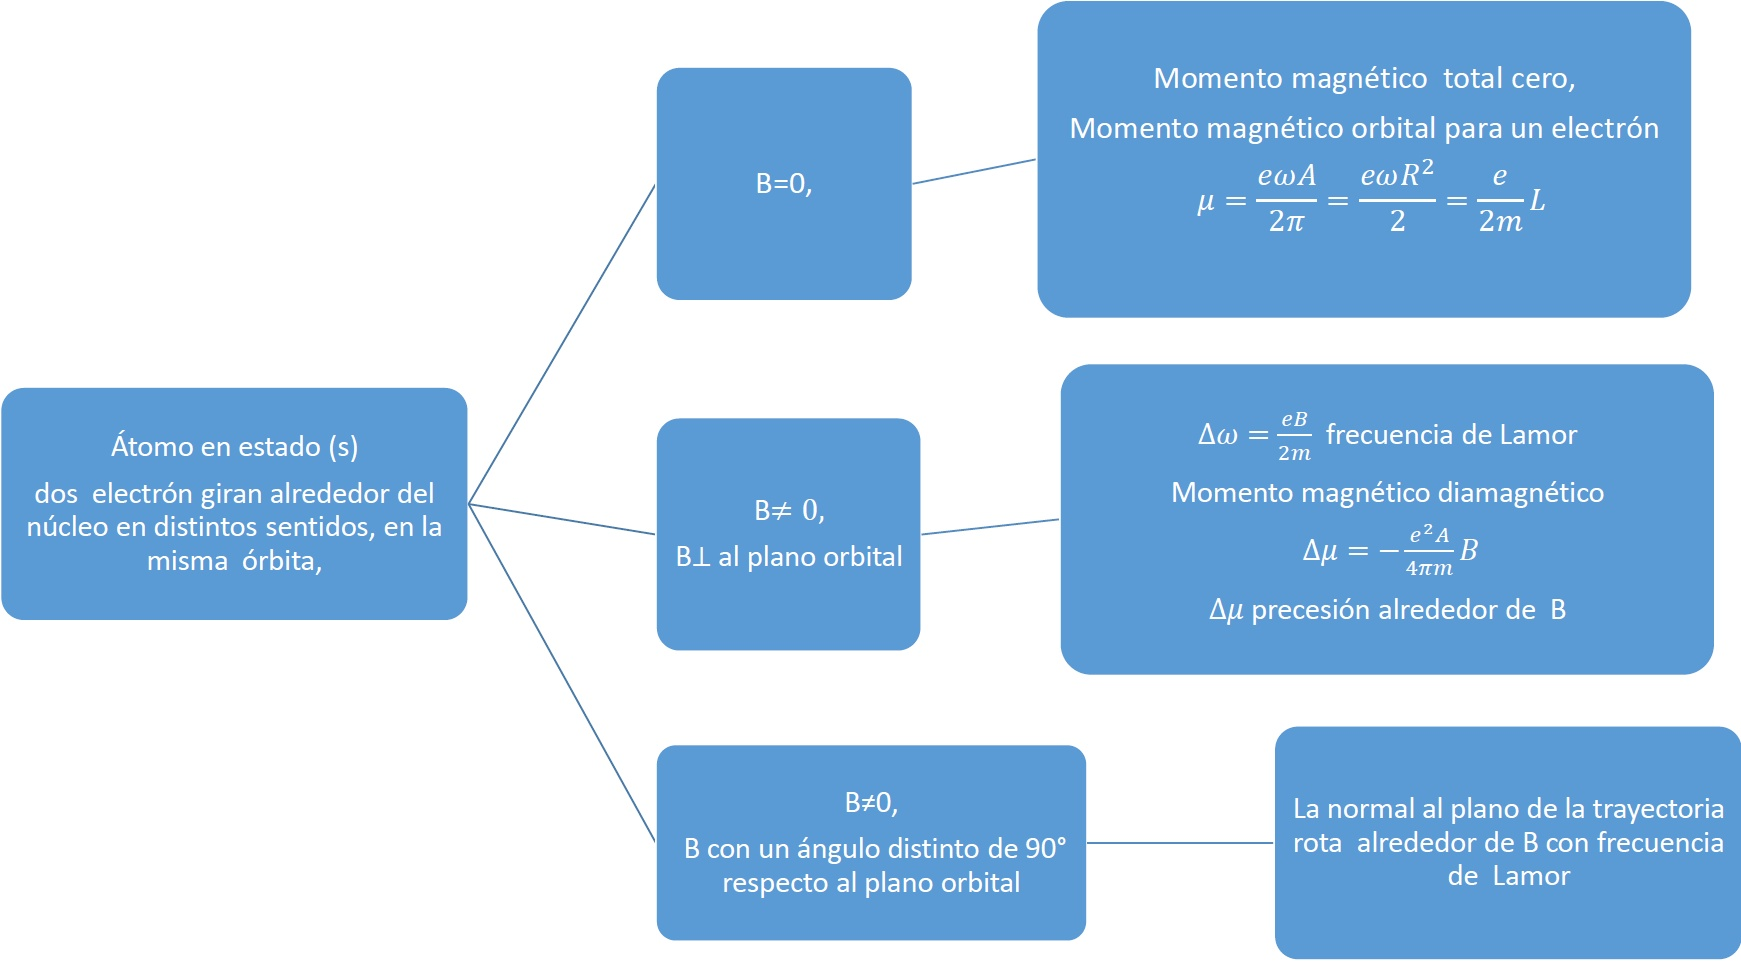
\includegraphics[width=1.0\textwidth]{./Figures/fig_s11}
	\caption{Teorema de Larmor}
	\label{fig:s11}
\end{figure}

El teorema afirma que si tenemos una partícula cargada orbitando en un campo de fuerzas centrales y le aplicamos un pequeño campo magnético, este produce un movimiento adicional de precesión que se superpone al movimiento original Dicho de otro modo el movimiento original es el mismo solo se agrega una precesión del momento magnético alrededor del vector campo magnético (en primer orden de $B$) con frecuencia de Larmor $\omega_{l}=\dfrac{eB}{2m}$.

El desarrollo anterior es clásico, si bien da una idea de la realidad las expresiones de la energía y del momento magnético no tuvieron en cuenta que no pueden tomar cualquier valor, ya que están cuantificadas Tampoco es posible definir una orbita en la trayectoria del electrón En el caso del momento angular cuántico es necesario tener en cuenta la cuantificación espacial, recordemos que puede encontrarse en $2l+1$ estados, luego la frecuencia de Larmor será, con $m=, \pm 1, \pm 2, \cdots, \pm l$

\begin{equation}
	\omega_{l}= \dfrac{eB}{2m_{e}}m \; \text{y la energía correspondiente} \;\Bb{\varepsilon}_{M}^{m}=\hbar\omega_{l}=\dfrac{e\hbar B}{2m_{e}}m
\end{equation}
La masa del electrón la hemos llamado $m_{e}$ para no confundir con el número cuántico $m$.

La distancia energética entre dos niveles próximos será:

\begin{equation}
	\Bb{\varepsilon}_{M}^{m}-\Bb{\varepsilon}_{M}^{m+1}=\dfrac{e\hbar B}{2m_{e}}
\end{equation}

Por medio de una onda electromagnética (ver figura \ref{fig:s12}) puedo entregarle al electrón, la energía correspondiente $\dfrac{e\hbar B}{2m_{e}}$ para que salte de un estado al otro, este expresión coincide con la clásica hallada anteriormente. Observemos que esta diferencia de energía no depende del nivel cuántico $m$. Si inicialmente estaba en equilibrio con el tiempo decaerá devolviendo la misma energía. Este fenómeno es el principio de la \textbf{resonancia magnética electrónica (rme)} y de la \textbf{resonancia magnética nuclear (rmn)}

\begin{figure}[H]
    \centering
    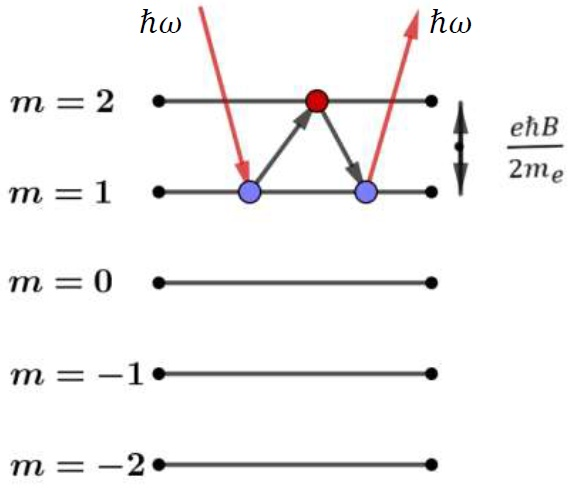
\includegraphics[width=0.5\textwidth]{./Figures/fig_s12}
	\caption{Frecuencia de Larmor}
	\label{fig:s12}
\end{figure}

\subsection{Paramagnetismo de Pauli}

Cuando los átomos se aproximan en un solido comienzan a interactuar entre ellos, sabemos que los electrones no pueden tener los mismos números cuántico, luego, no queda otra que crear nuevos niveles Como la cantidad de átomos es elevada se forma un continuo de niveles, llamada bandas de energía Zona donde deambulan los electrones libremente, sin saber a que átomo, pertenecen ya que son indistinguibles, similar un gas de electrones, o gas de Fermiones. 

Veamos un calculo simple, si tenemos $N$ átomos cada uno de ellos aporta un nivel, en 55,85 gr de $Fe$ hay el numero de Avogadro de átomos $N=6,023\times 10^{23}$ luego tenemos el mismo número de niveles. Adenás, por el Principio de exclusión de Pauli, tendremos 2 electrones por nivel de energía. En la figura \ref{fig:s13} se observan los niveles en los átomos alejados y
como a partir de un distancia $d_{0}$ comienza la aparición de las bandas. Es claro que los orbitales más externos son los primeros en interactuar y solaparse, en el esquema el $4s$
después el $3d$.

Se genera un continuo de niveles, la diferencia de energía entre niveles es pequeña En este caso los electrones se pueden excitar fácilmente y pasar de un nivel lleno a los vacíos inmediatos, explicando de esta manera la conductividad eléctrica y térmica La importante cantidad de niveles en la banda permite la absorción de radiación de cualquier longitud de onda, y también su emisión, explicación  ésta de su alta reflectividad.

El área debajo de la curva es igual al número total disponible de niveles de energía en una banda

\begin{figure}[H]
    \centering
    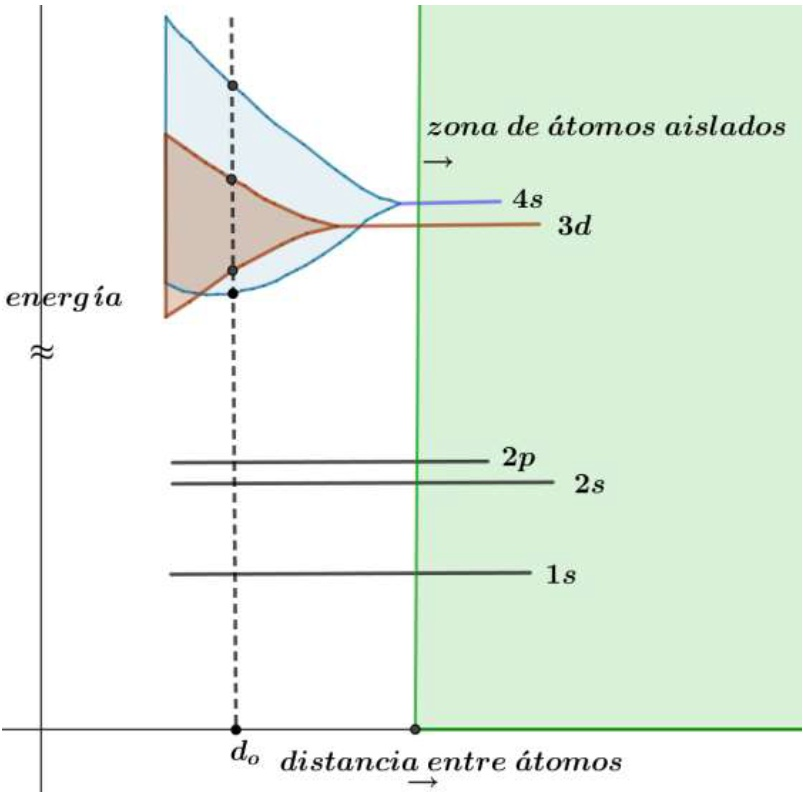
\includegraphics[width=0.8\textwidth]{./Figures/fig_s13}
	\caption{Formación de bandas de energía}
	\label{fig:s13}
\end{figure}

En la figura \ref{fig:s14} se observa la densidad de estados para las zonas indicadas La banda $3d$ tiene una densidad de estados mayor que $4s$ porque hay cinco niveles en $3d$ por átomo, cada uno con una capacidad de 10 electrones. Mientras que en la $4s$ tenemos $2$ electrones.

Este continuo de niveles nos posibilita hablar de una densidad de niveles o estados en función de la energía,(en esta parte del apunte $E$ es energía no campo eléctrico) comúnmente designada:

\begin{equation}
\begin{aligned}
	\rho(E)&= \dfrac{\text{n° de estados con energía E}}{\text{n° de estados totales de energía por u. de volumen}} \\
	&= \dfrac{(8 \pi \sqrt{2} m )^{\frac{3}{2}}}{h^{3}}\sqrt{E}
\end{aligned}
\end{equation}

Donde $\rho(E)dE =$ n° de estados entre $E$ y $E+dE$, en la unidad de volumen, la cantidad total de estados será $\int_{0}^{E} \rho(E)dE$

La densidad de estados nos da el número de estados de energías por unidad de energía comprendidos entre dos niveles energéticos entre sí, $E$ y $E+dE$. \textbf{Estos estados pueden estar ocupados por electrones o estar vacantes}.
 
Las líneas de rayas, en el esquema, muestran el \textbf{nivel de Fermi} que es el término que indica el nivel superior del conjunto de valores de la energía de los electrones a la temperatura de cero absoluto, la energía correspondiente al nivel de Fermi se llama \textbf{energía de Fermi} ($E_{F}$). A temperaturas mayores a el cero absoluto, existirá una cierta fracción de electrones determinada por la función de Fermi, por encima del nivel de Fermi.

La función de Fermi $f(E)$ nos da la probabilidad de que un estado de una dada energía sea
ocupado por un electrón a una data temperatura, es:

\begin{equation}
	f(E)=\dfrac{1}{exp\left(\dfrac{E-E_{F}}{kT}\right)  + 1} = \dfrac{\text{n° de electrones en el estado E}}{\text{n° total de electrones posibles en el estado E}}	
\end{equation}

Los iones del metal que comparten los electrones deben ser diamagnéticos, ya que al perder sus electrones se parecen al gas noble mas próximo.

\begin{figure}[H]
    \centering
    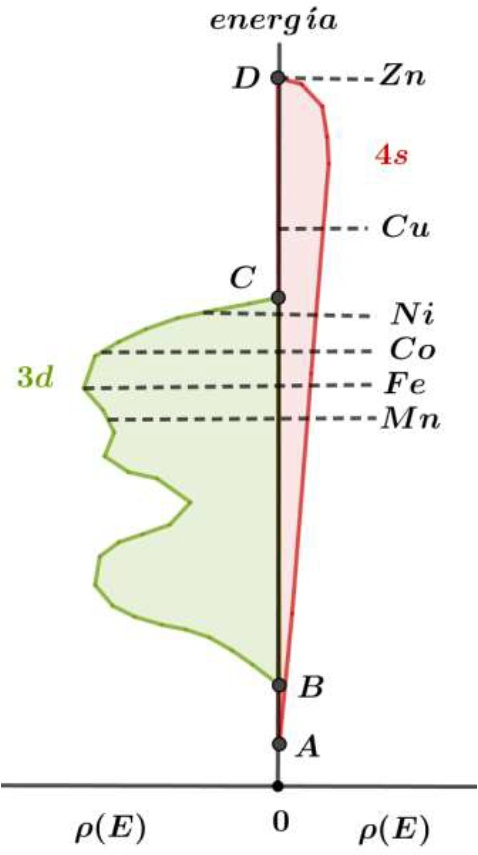
\includegraphics[width=0.5\textwidth]{./Figures/fig_s14}
	\caption{Densidad de estados para diversos elementos.}
	\label{fig:s14}
\end{figure}

Analicemos la función Fermi $f(E)=\dfrac{1}{exp \left(\dfrac{E-E_{F}}{kT}\right)+1 }$, vemos en ella que si la temperatura $T\rightarrow 0$, hay dos posibilidades, si $E < E_{F}$ el resultado es $1$, la certeza, todos los niveles ocupados, por el contrario si $E<E_{F}$ es cero la probabilidad de encontrar un electrón por arriba del nivel de Fermi.

\begin{equation}
\begin{aligned}
	\rho(E)f(E) &= \dfrac{1}{exp\left(\dfrac{E-E_{F}}{kT}\right)+1 } \\
	&= \dfrac{\text{n° de estados x n° de $e^{-}$ en el estado E}}{\text{n°total de estados x  n° total de $e^{-}$ posibles en el estado E}}	
\end{aligned}
\end{equation}


Luego $\rho(E)f(E)dE$ nos da el número de electrones por unidad de volumen con energía en el intervalo $E , \; E+dE$. Los niveles de energía que se manejan comúnmente son muy chicos comparados con la energía de Fermi, por ejemplo en la figura \ref{fig:s15} se ve que la energía de Fermi para el cobre es $E_{F}(Cu)\approx 7eV$ mientras que la energía térmica a $300{^{o}}K$ es de $0,026eV$. Esto nos indica que la energía térmica comúnmente usada, solo puede interactuar con los electrones próximos a la energía de Fermi.

\begin{figure}[H]
    \centering
    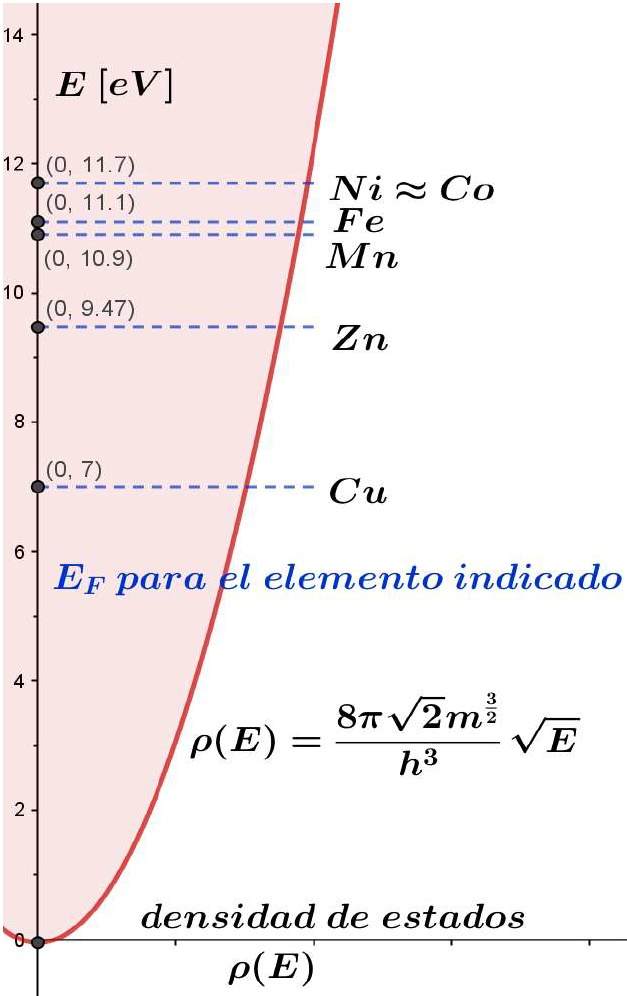
\includegraphics[width=0.6\textwidth]{./Figures/fig_s15}
	\caption{Densidad de estados Paragamagnetismo de Pauli}
	\label{fig:s15}
\end{figure}

El modelo de Pauli es válido para materiales en los que los electrones son libres y forman una capa de conducción Se puede aplicar a la mayoría de los metales paramagnéticos Podemos pensar que en ausencia de campo magnético externo, sobre un metal, en cada sub banda se colocan el número total de electrones dividido dos. La
mitad de ellos con el espín hacia arriba y la otra mitad con el espín hacia abajo, luego el momento magnético será:

\begin{equation}
	\mu_{p}= (n\uparrow - n\downarrow)\mu_{B} = 0
\end{equation}

Siendo $n\uparrow$ el número de electrones de conducción con espín hacia arriba en la unidad de volumen cuando no hay campo magnético externo ($\V{B}=0$), como se menciono, la parábola de densidad de energía se dividida en dos; una formada por los espines hacia arriba y la otra con los espines como se muestra en la figura \ref{fig:s16}, Si ahora se coloca un campo $\V{B}\neq 0$, los electrones próximos a la energía de Fermi aumentan su energía en $\mu_{B}B$ si sus espines coinciden con el sentido del campo exterior, Ya que con un espín alineado con el campo tienen menos energía que los no
alineados. Luego, en presencia de campo debe aumentar el número de espines alineados al campo y decrecer el número de los no alineados en  $-\mu_{B}B$. De esta manera las dos semibandas se desplazan una de otra en  $2\mu_{B}B$ como se observa en la misma figura \ref{fig:s16}. Como el sistema tiende al mínimo de energía, una porción de electrones de la derecha del esquema debe pasar al de la izquierda, modificando su espín como observamos en el esquema. Como resultado surge un momento magnético en la dirección del campo externo $\V{B}$.

\begin{figure}[H]
    \centering
    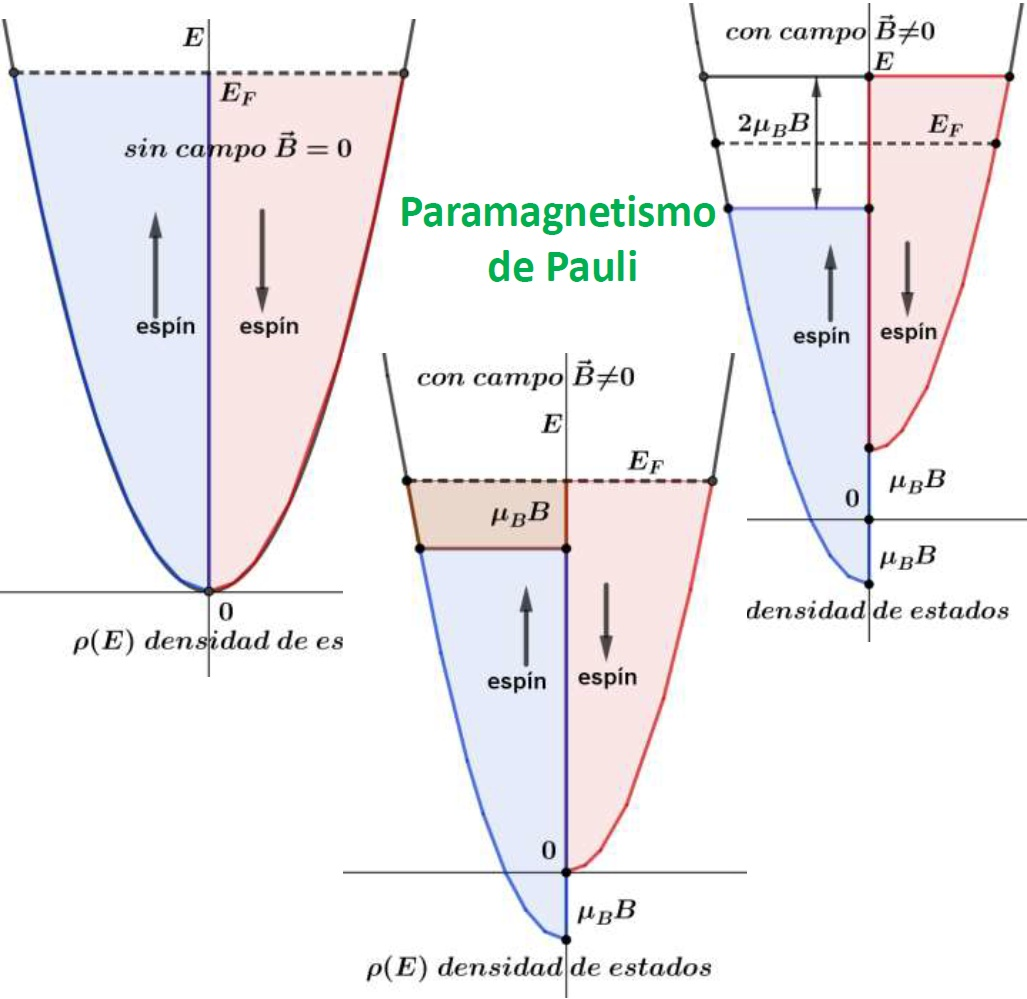
\includegraphics[width=0.9\textwidth]{./Figures/fig_s16}
	\caption{Desdoblamiento energético de la densidad de estados}
	\label{fig:s16}
\end{figure}





\section{Paramagnetismo en sólidos y gases}

Recapitulemos: Como hemos visto, en un átomo, los únicos electrones que pueden contribuir al momento magnético total del átomo son los que están en capas incompletas, generalmente electrones de valencia, dado que en las capas electrónicas completas el momento magnético orbital y de espín es cero. Como la mayoría de los átomos tienen capas incompletas, también tendrán momento magnético no nulo. Pero esto sólo es cierto para átomos libres, no para átomos dentro de un sólido, ligados entre sí por fuerzas de enlace. La razón es que la energía de intercambio de los electrones de átomos vecinos es normalmente mínima cuando sus espines están dispuestos de forma antiparalela y de ahí que el momento dipolar total de la molécula sea nulo.

En los cristales iónicos los electrones externos de un átomo son transferidos para completar la capa de su vecino, ambos iones tendrán capas electrónicas completas y tendremos un momento magnético nulo. Por tanto, el paramagnetismo sólo se dará en sólidos formados por átomos con capas incompletas, además de las ocupadas por electrones de valencia.

Existen cinco grupos de elementos donde ocurre esto

\begin{itemize}
	\item Grupo del $Fe$ - capa $3d$ incompleta
	\item Grupo del $Pd$ - capa $4d$ incompleta
	\item Lantánidos - capa $4f$ incompleta
	\item Grupo del $Pt$ - capa $5d$ incompleta
	\item Actínidos - capa $5f$ incompleta
\end{itemize}

Además, los metales muestran también \textbf{paramagnetismo debido a los electrones de conducción}. Este paramagnetismo muestra la propiedad de que la susceptibilidad es prácticamente independiente de la temperatura. Los materiales empleados para aplicaciones prácticas están hechos de sales de hierro o de tierras raras.

\subsection{Susceptibilidad paramagnética de los electrones de conducción}

Se observa experimentalmente como casi todos los metales (a excepción de Pd y Ti) muestran un efecto paramagnético débil y poco dependiente de la temperatura. La teoría clásica de electrones libres es incapaz de aportar una explicación satisfactoria de la susceptibilidad paramagnética de los electrones de conducción. Como cada electrón tiene un momento magnético asociado de un magnetón de Bohr, podría pensarse que la contribución de los electrones de conducción a la susceptibilidad paramagnética sería del tipo Curie :

\begin{equation}
	M=\frac{N\mu_B^{2}}{k_{B}T}\,B
\label{eq:SusParCurie}
\end{equation}

Expresión de la fórmula \ref{eq:SusParCurie} está contra de la observación experimental de que la susceptibilidad es independiente de la temperatura en la mayoría de los metales.

Pauli demostró que la aplicación de la estadística de Fermi-Dirac aporta a la teoría las correcciones necesarias.

\begin{figure}[H]
    \centering
    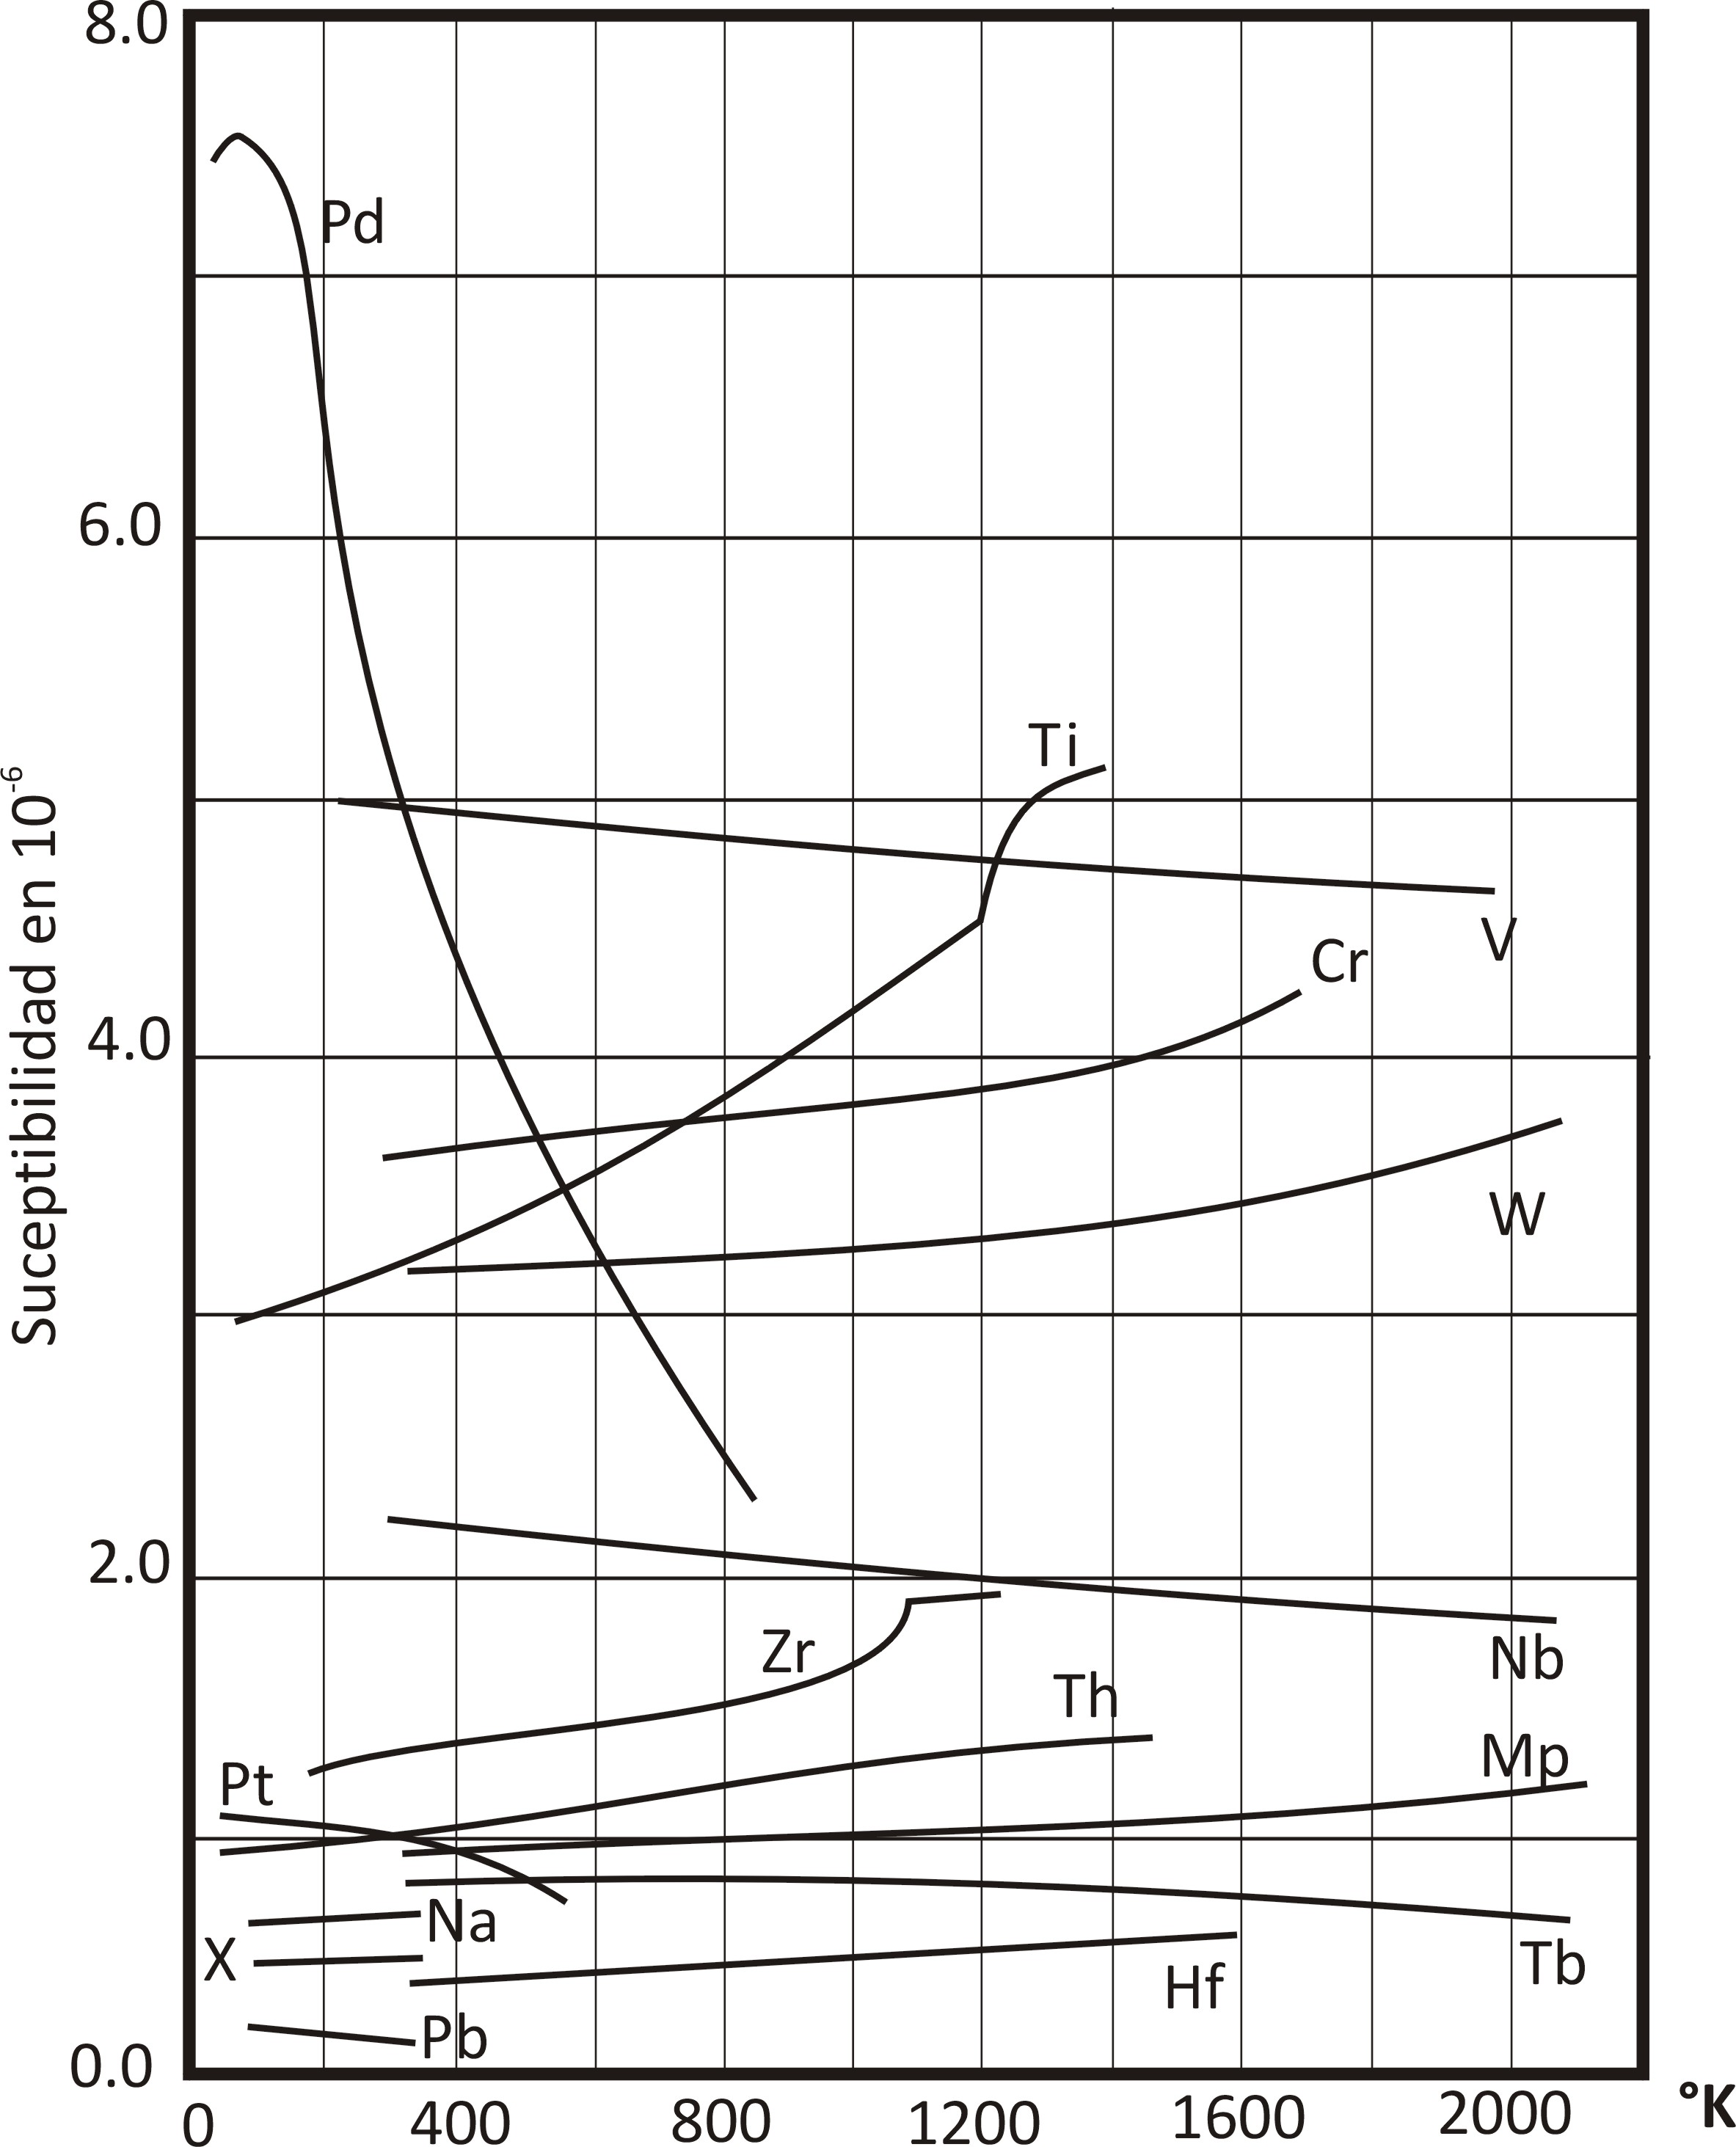
\includegraphics[width=0.8\textwidth]{./Figures/Suceptibilidad}
	\caption{Suceptibilidad de diversos elementos}
	\label{fig:Suceptibilidad}
\end{figure}

Abordemos en primer lugar una explicación cualitativa:

Para un solo electrón desapareado, en presencia de un campo magnético exterior $B$ y con solo el momento angular de espín tendremos una energía: $2\mu_{B}B$

\begin{figure}[H]
    \centering
    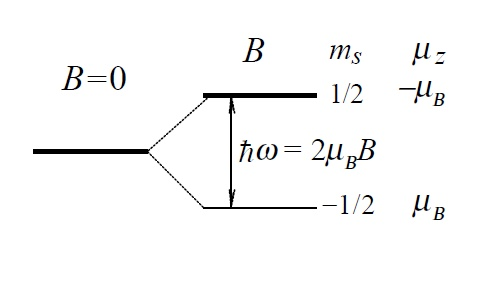
\includegraphics[width=0.6\textwidth]{./Figures/dosNiveles}
	\caption{Desdoblamiento de la energía por el campo $B$}
	\label{fig:dosNiveles}
\end{figure}

En el estado de menor energía, el momento magnético es paralelo al campo. Como el sistema tiene sólo 2 niveles, sus poblaciones en equilibrio térmico son (estadística de Maxwell-Boltzmann)

\begin{equation}
\frac{N\uparrow}{N}=\frac{e^{\frac{\mu_{B}B}{k_{B}T}}}{e^{\frac{\mu_{B}B}{k_{B}T}}+e^{\frac{-\mu_{B}B}{k_{B}T}}} \quad \text{y} \quad \frac{N\downarrow}{N}=\frac{e^{-\frac{\mu_{B}B}{k_{B}T}}}{e^{\frac{\mu_{B}B}{k_{B}T}}+e^{\frac{-\mu_{B}B}{k_{B}T}}}
\end{equation}

Con $N\uparrow$ y $N\downarrow$ las poblaciones de espines en los niveles $+1/2$ y $-1/2$ y $N=N\uparrow+N\downarrow$ los átomos por unidad de volumen.

La magnetización resultante $M$ para $N$ átomos por unidad de volumen será entonces:

\begin{equation}
M=(N\uparrow-N\downarrow)\mu_{B}=N\mu_{B}\frac{e^{X}-e^{-X}}{e^{X}+e^{-X}}=N\mu_{B}\,tanh(X) \quad,\quad  X=\frac{\mu_{B}B}{k_{B}T}
\end{equation}

Para $X\ll1$, $tanh(X)\approx X \longrightarrow M\approx M_{\mu_{B}}\big(\frac{\mu_{B}B}{k_{B}T}\big)$

Según esta ecuación, la probabilidad de que un electrón de conducción se oriente con su espín paralelo a $B$ excede en $\sim\big(\frac{\mu_{B}B}{k_{B}T}\big)$ a que lo haga en la orientación antiparalela. Para $N$ electrones de conducción por unidad de volumen, el momento magnético total es $\sim \big( \frac{\mu_{B}^{2}B}{k_{B}T}\big)$ y coincide con la teoría clásica. Sin embargo, muchos electrones de conducción tienen una probabilidad nula de orientarse al aplicar un campo, ya que muchos orbitales de espín paralelo están ocupados. Sólo los electrones dentro de un dominio $\sim k_{B} T$ alrededor del nivel de Fermi $T_{F}$ tendrán la posibilidad de ser orientados con el campo. Por tanto sólo la fracción $T/T_{F}$ del número total de electrones contribuye a la susceptibilidad:

\begin{equation}
 M \approx \frac{\mu_{B}^{2}}{k_{B}T}\, B\, \frac{T}{T_{F}} = \frac{\mu_{B}^{2}}{k_{B}T_{F}}\, B
\end{equation}

dando lugar a una susceptibilidad independiente de la temperatura y del orden de magnitud observado experimentalmente.

Calculemos la susceptibilidad paramagnética de un gas de electrones libres como el que hay en el seno de un
conductor metálico para $T << T_{F}$ :

%\begin{figure}[H]
%    \centering
%    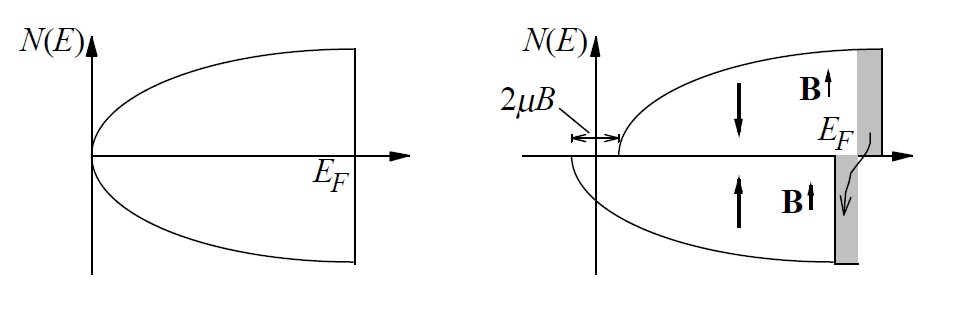
\includegraphics[width=0.8\textwidth]{./Figures/dosNivelesGas}
%	\caption{Densidad de estados en la estadística de Fermi - Dirac}
%	\label{fig:dosNivelesGas}
%\end{figure}



En este caso tendremos una estadística de Fermi –Dirac y las concentraciones $N\uparrow$ y $N\downarrow$ se podrán expresar como:

\begin{equation}
  N\uparrow\downarrow = \frac{1}{2} \int_{\mu_{B}B}^{E_{F}} f(E)D(E\pm \mu_{B}B dE \approx 
            \frac{1}{2} \int_{\mu_{B}B}^{E_{F}} f(E)D(E) dE \pm \frac{1}{2}\mu_{B}B D(E_{F}) 
\end{equation}

Con lo que resulta:

\begin{equation}
  M = (N\uparrow-N\downarrow)\mu_{B} = \mu_{B}^{2}D(E_{F})B = \frac{3N\mu_{B}^{2}}{2k_{B}T_{F}}B
\end{equation}

conocida como \textbf{magnetización de espín de Pauli} de los electrones de conducción con

\begin{equation}
  D(E_{F}) = \frac{3N}{2E_{F}} = \frac{3N}{2Ek_{B}T_{F}} 
\end{equation}

Al calcular este resultado se ha supuesto que el movimiento espacial de los electrones no está afectado por el campo magnético. Sin embargo, las funciones de onda son modificadas por el campo magnético y los electrones libres crean un momento diamagnético igual a $-1/3$ del momento paramagnético (según Landau).
Por tanto, la magnetización total de un gas de electrones libres es igual a:

\begin{equation}
  M = \frac{N\mu_{B}^{2}}{k_{B}T_{F}}B \quad \text{y} \quad \chi=\frac{N\mu_{0}\mu_{B}^{2}}{k_{B}T_{F}} 
\end{equation}

Al comparar esta fórmula con los resultados experimentales hay que tener en cuenta:

\begin{itemize}
	\item El magnetismo de los iones.
	\item Los efectos de la banda $\rightarrow$ aumento de la susceptibilidad.
	\item La interacción electrón-electrón
\end{itemize}
La susceptibilidad magnética de los metales de transición (con capas electrónicas incompletas) es bastante más elevada que para los metales alcalinos. Esto hace suponer que la densidad de estados en la ecuación $D(E)$ es anormalmente elevada en los metales de transición, lo cual se deduce efectivamente a partir de la teoría de bandas.

El paramagnetismo de Pauli es un efecto débil solo una pequeña fracción de electrones con energía cercana a $E_{F}$ contribuyen al paramagnetismo de Pauli. Al hallar la magnetización se supuso que el campo magnético no influye sobre el movimiento espacial de los electrones, cosa que no es del todo cierta, como veremos mas adelante.

\subsection{Resumen de Paramagnetismo}

\begin{itemize}
	\item En un átomo tanto el momento de spin como el angular aportan al paramagnetismo aunque generalmente el aporte del espín es más importante.
	\item En átomos con niveles completamente ocupados, los momentos magnéticos se compensan y no
hay momento magnético resultante.
	\item El momento magnético de espín puede estar en dirección paralela al campo exterior o antiparalela a
este
	\item Son paramagnético todos los átomos y moléculas que poseen un número impar de electrones, pues presentan un momento magnético. El spin total del sistema no debe ser nulo, Ejemplo: átomos libres de sodio, oxido nítrico gaseoso (NO).
	\item También son paramagnéticos todos los átomos y iones libres con una capa interna incompleta, ejemplo elementos de transición, $Mn^{2+}$, $Gd^{3+}$
	\item Todas las sustancias a altas temperaturas son diamagnéticas o paramagnéticas.
	\item El momento magnético fundamental es el magnetón de Bohr ($\mu B$), que tiene una magnitud de  $9.27x10^{-24} Am^{2}$. Para cada electrón en el átomo el momento magnético de espín es $\pm\mu B$, adicionalmente la contribución del momento magnético de orbital es igual a $m_{l}\mu B$, siendo $m_{l}$ el número cuántico magnético del electrón.
\end{itemize}


\section{Diamagnetismo atómico, iónico, molecular}

\begin{itemize}
	\item El diamagnetismo fue descubierto por S. Justinus Brugmans. En 1778 observo que el bismuto y el antimonio son repelidos por los campos magnético. Este es un claro comportamiento diamagnético puesto que $\chi_{v}<0$.
\end{itemize}

\textbf{Explicación clásica del diamagnetismo:}

\begin{itemize}
	\item Conocemos el comportamiento eléctrico de una espiral por la que circula una corriente en un campo magnético. De acuerdo a la ley de Lenz, al variar el flujo magnético sobre un circuito eléctrico, surge en el circuito una fem inducida que produce una variación de la corriente. La corriente generada produce un campo magnético adicional que se opone al original. Un electrón en su órbita es considerado como una corriente eléctrica.
	\item La diferencia con la espira común es que la resistencia del circuito orbital es nula, por eso se conserva el campo magnético mientras exista el exterior.
	\item El momento magnético generado por esta corriente (la creada por la fem) es precisamente la responsable del diamagnetismo, generando el momento diamagnético y explicando porque los átomos diamagnéticos se alejan del campo magnético aplicado.
	\item De acuerdo a la explicación previa, es claro que todos los átomos deben poseer diamagnetismo, por ser muy débil es solo observable cuando todos los demás tipos de magnetismo son inexistentes. Átomos netamente diamagnéticos son Bi, Cu, Ag, Au.
\end{itemize}




\subsection{Diamagnetismo (clásico), teoría de Paul Langevin 1905}

Como se comentó, el efecto diamagnético es sumamente pequeño, por esta razón se estudia el diamagnetismo en los átomos o moléculas que no tienen momento magnético propio, no son paramagnéticos, estado $s$ Luego los átomos que tratamos deben tener en su ultima capa dos electrones. Sabemos que el electrón no describe trayectorias bien definidas en su giro alrededor del núcleo, pero, en la deducción de la expresión del diamagnetismo suponer la existencia de una órbita determinada, da una buena concordancia con los datos experimentales. Vimos anteriormente, en el tema frecuencia de Larmor, que el momento magnético de un electrón girando en una orbita determinada al rededor del núcleo es $\mu=iA= e\dfrac{\omega}{2\pi}A$, por tanto un cambio en $\omega$ genera una variación en $\mu$, $\Delta\mu=e\dfrac{\Delta}\omega{2\pi}A$ reemplazando la frecuencia de Larmor $\Delta\omega=\dfrac{eB}{2m}$ encontrada previamente tenemos

\begin{equation*}
	\Delta\mu=\dfrac{e^{2}A}{4\pi m}B
\end{equation*}

Luego, el diamagnetismo aparece como oposición al campo magnético externo. $B$ engendra el momento magnético adicional $\Delta\mu$ dirigido en contra de el, o sea de campo externo Este efecto no es momentáneo, existe siempre que el campo este presente ya que la supuesta corriente $i$ no es real y la espira no tiene resistencia.

Cuando se dedujo la expresión de Larmor se supuso una órbita plana, tratemos de generalizar la expresión hallada previamente a un caso más real. Sabemos que los electrones en un átomo no magnético, se mueven en órbitas esféricas, supongamos de radio $R$ no en una circunferencia de radio $r$ ver esquema electrones Si el campo $B$ está alineado con $zy$ y suponemos que todas las direcciones de movimiento son igualmente probables, entonces el valor medio de las coordenadas $\langle x^{2}\rangle=\langle y^{2} \rangle =\langle z^{2} \rangle$ son independientes e igualmente distribuidas por tanto, ver figura \ref{fig:s17}


\begin{figure}[H]
    \centering
    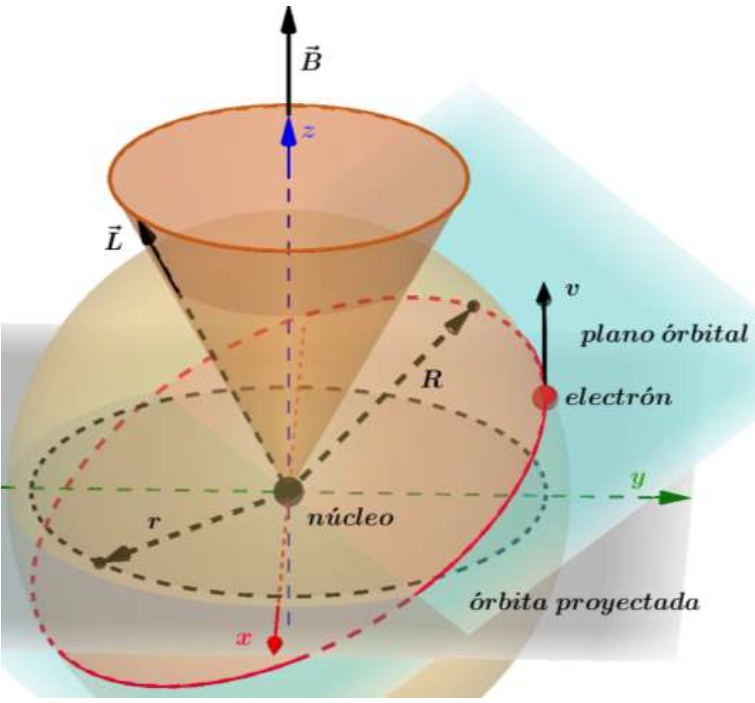
\includegraphics[width=0.8\textwidth]{./Figures/fig_s17}
	\caption{Diamagnetismo clásico}
	\label{fig:s17}
\end{figure}

\begin{equation}
\begin{aligned}
&\langle R^{2} \rangle = \langle x^{2}\rangle + \langle y^{2} \rangle + \langle z^{2} \rangle \quad \text{luego} \quad \langle R^{2} \rangle = 3\langle x^{2}\rangle\rightarrow \langle x^{2} \rangle = \dfrac{\langle R^{2}\rangle}{3} \\
& \text{y como} \quad \langle x^{2}\rangle = \dfrac{r^{2}}{2} \rightarrow \dfrac{\langle r^{2} \rangle}{2}=\dfrac{\langle R^{2} \rangle}{3} \quad \text{esntonces resultará}\\
& \qquad \langle r^{2} \rangle= \dfrac{2\langle R^{2} \rangle}{3}
\end{aligned}
\end{equation}

y $\Delta\mu$ será:

\begin{equation}
\begin{aligned}
\Delta \mu = -\dfrac{e^{2}A}{4\pi m}B &= -\dfrac{e^{2}\pi r^{2} }{4\pi m}B = -\dfrac{e^{2}\langle r \rangle^{2}}{4m} &= -\dfrac{e^{2}R^{2}}{6M}B
\end{aligned}
\end{equation}

Donde $R^{2}$ es el radio promedio de una órbita que puede tomar todas las direcciones posibles con respecto al campo $B$. Hasta ahora hemos considerando un solo electrón en el átomo. Si el átomo contiene $Z$ electrones $\Delta\mu$(por átomo) $=-\dfrac{Ze^{2}B}{6m}\sum R_{i}^{2}$.

Donde $R_{i}$ es el radio de la enésima órbita La expresión $\sum R_{i}^{2}$ puede ser reemplazada por $ZR^{2}$ donde $R^{2}$ es el promedio de los cuadrados de varios radios atómicos. Para pasar a una expresión por volumen, sabemos que el número de átomos por unidad de volumen es $N\rho A$ donde $N$ es el número de Avogadro, $\rho$ la densidad y $A$ el peso atómico, luego

\begin{equation}
	\Delta\mu\text{(por $cm^3$)} =- \left( \dfrac{N\rho}{A}\right) \dfrac{Ze^{2}R^{2}B}{6m}
\end{equation}


mientras que la susceptibilidad diamagnética es:

\begin{equation}
	\Delta\mu\text{(por $cm^3$)} =- \left( \dfrac{N\rho}{A}\right) \dfrac{Ze^{2}R^{2}B}{6m}
\end{equation}

Vemos que en general la susceptibilidad diamagnética no depende de la temperatura, sin embargo, a temperaturas muy bajas no es del todo cierto, también observamos que crece con $Z$. En la figura \ref{fig:s17} se pone de manifiesto el vector $L$ girando alrededor de el campo $B$ con la frecuencia de Larmor, observamos el plano orbital que no coincide con el $x$, y también se representa la esfera de radio $r$ donde coexisten la órbita de los dos electrones.

\subsection{Diamagnetismo (clásico) detalle de cómo se suman los momentos diamagnéticos}

Como fue comentado estamos trabajando en átomos que no son paramagnéticos, o sea que tenemos dos electrones orbitando tal como se muestra en la figura \ref{fig:s18}, moviéndose en sentidos opuestos. Luego los momentos angulares orbitales $L$ son opuestos y el momento orbital total del átomo es cero (vectores negros en los esquemas) De igual manera tenemos dos momentos magnéticos opuestos en el mismo átomo (vector verde). Al introducir un campo magnético externo $B$ se modifican las velocidades,(en distintos sentidos) de los dos electrones que giran en sentido contrario, generando cada uno de ellos un momento magnético $\Delta\mu$ (vector fucsia que se opone al campo, ley de Lenz). El momento diamagnético total de
átomo será $\Delta\mu_total = 2\Delta\mu$. Queda claro que todos los átomos son diamagnéticos, pero para poder observarlos el grado de su ionización debe ser tal que se asemeje al gas noble mas próximo, ya que este ultimo tiene sus envolturas electrónicas completas. El $Na$ tiene número atómico 11 y la estructura electrónica es $[Ne]3s^{1}$ si se ioniza pasa a tener la estructura del $Ne$ que es $1s^{2}2s^{2}2p^{6}$ y al tener la última capa completa no es paramagnético, luego es posible
observar el diamagnetismo. El diamagnetismo se pudo explicar clásicamente y coincide bien con los resultados experimentales, sin embargo el momento diamagnético permanece siempre que el campo exista, cosa que no sucede cuando uno aplica la ley de Lenz en electrodinámica.


\begin{figure}[H]
    \centering
    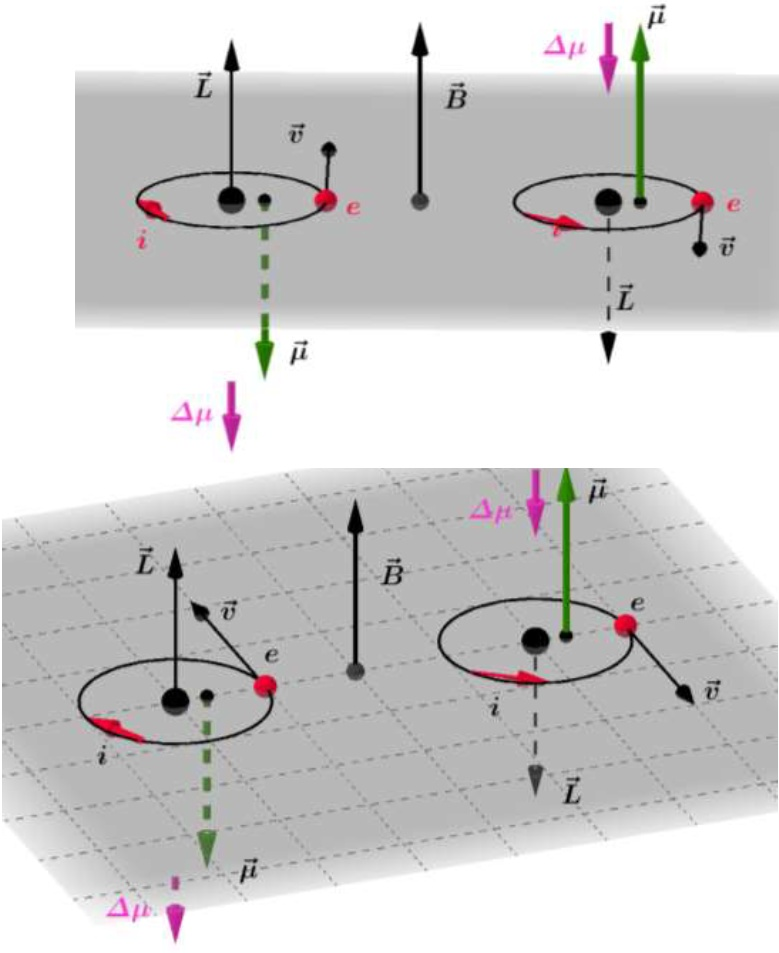
\includegraphics[width=0.8\textwidth]{./Figures/fig_s18}
	\caption{Suma de momentos diamagnéticos}
	\label{fig:s18}
\end{figure}

\subsection{Resumen de diamagnetismo}

\begin{itemize}
	\item El diamagnetismo es una propiedad de la materia en cualquier estado. El comportamiento diamagnético se observa claramente en los sistemas atómicos, iónicos y moleculares que contengan todos sus electrones apareados y que tengan orbitales completamente llenos. Es decir los espines de los electrones del último nivel se deben encontrar apareados.

	\item De lo mencionado es claro que puede ser observado el diamagnetismo en todas las sustancias que tengan estructura de gas noble (8 electrones) como $H^{-}, Li^{+}, Na^{+}, Ca^{2+}, Ti^{4+}$... ; o bien (18 electrones): $Cu^{+}, Ag^{+}, Hg^{2+}$... o perdiendo dos electrones y quedando el átomo con dos cargas positiva (+2) i.e. (20 electrones): $Sn^{2+}, Pb^{2+}$, en el caso del antimonio de estructura $[Kr]\, 4d^{10}\, 5s^{2}\, 5p^{3}$, eliminando 3 electrones $Sb^{3+}$, cumplimos las condiciones.
	
	\item Como el momento inducido sólo depende del tamaño y de la forma de los orbitales en las capas completas y esto, no depende de la temperatura, luego el diamagnetismo depende poco de la temperatura. A temperaturas muy bajas, los metales (ojo en sólidos metálicos) el diamagnetismo presenta fuertes variaciones de $\chi$ (susceptibilidad ) con la temperatura T, y violentas oscilaciones al variar poco valor de $\overrightarrow{H_{0}}$ que se llama efecto Hass – van Alphen.

	\item Ya que el diamagnetismo es función de la distribución electrónica dentro de un átomo, ion o molécula y es causado por la interacción del campo aplicado sobre los orbitales llenos de electrones, va a ser mas importante el diamagnetismo en los átomos con mayor numero de electrones.

	\item Los spines de los electrones no tienen nada que ver con este momento inducido, estos permanecen firmemente acoplados.
\end{itemize}

En la figura \ref{fig:s19} Otra manera de encontrar la relación entre $r$ (órbita en el plano perpendicular al campo) y $R$ (radio de una órbita cualquiera). En nuestro caso mostramos, ver esquema, el plano orbital inclinado un ángulo $\theta$ respecto al $B$. Se debe reemplazar en la expresión $\mu=\dfrac{e\omega \langle r^{2} \rangle}{2}$ el valor medio de $r^{2}$ por una función de $R$.

Para ello $\langle r^{2} \rangle= \langle R^{2} Sin^{2}(\theta)\rangle = R^{2} \dfrac{\int Sin^{2} \theta dA}{A}$ donde:

\begin{equation}
\begin{aligned}
&dA= (2\pi r Sin(\theta) ) R d\theta = 2 \pi R^{2} sin(\theta) d\theta \\
&\langle r^{2} \rangle = R^{2} \dfrac{\int Sin^{2}(\theta) dA}{A} \\
&=R^{2} \dfrac{\int_{0}^{\frac{\pi}{2}}Sin^{2}\theta(2\pi R^{2} Sin\theta)d\theta}{2\pi R^{2}}\\
&=R^{2}\int_{0}^{\frac{\pi}{2}} Sin^{3}\theta d\theta=R^{2}\left[ -Cos(\theta)+\dfrac{Cos^{3}\theta}{3}\right] _{0}^{\frac{\pi}{2}}= \dfrac{2R^{2}}{3}
\end{aligned}
\end{equation}

\begin{figure}[H]
    \centering
    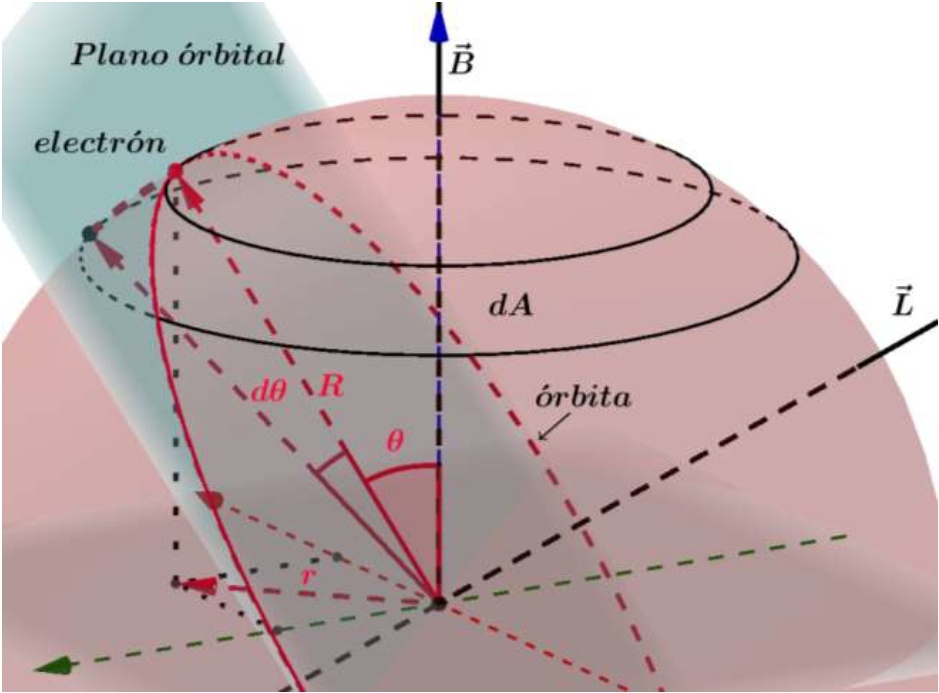
\includegraphics[width=1.0\textwidth]{./Figures/fig_s19}
	\caption{Relación de radios orbitales $R$ y $r$}
	\label{fig:s19}
\end{figure}

En la figura \ref{fig:s20} vemos una manera alternativa de llegar al mismo resultado anterior aplicando las ecuaciones de Maxwell. Supongamos como anteriormente que el electrón gira en su órbita. Las ecuaciones que responden a la aplicación de un campo magnético uniforme, lentamente aplicado, de tal modo que $\dPv{B}{t}$ no sea cero, es

\begin{equation*}
	\Rotor{E}= -\dPv{B}{t} \quad \text{y} \quad \Diver{B}=0
\end{equation*}


Si $\V{B}=(0,0,B)\Rightarrow \Rotor{E}=\left( 0,0,\dP{B}{t} \right) = \dP{B}{t} \hat{k}\quad$ mientras que:


\begin{equation}
	\Rotor{E}_{z}= \left( \dP{E_{y}}{x} - \dP{E_{x}}{y} \right)\hat{k} = \dP{B}{t}
\end{equation}

Cualquiera sea la órbita el campo eléctrico tiene componentes en $x$ e $y$, Tratamos de hallar el campo $\V{E}$, para ello integramos:

\begin{equation}
	\int \Rotor{E} \cdot d\V{S}= -\int \dPv{B}{t} \cdot d\V{S}
\end{equation}



\begin{figure}[H]
    \centering
    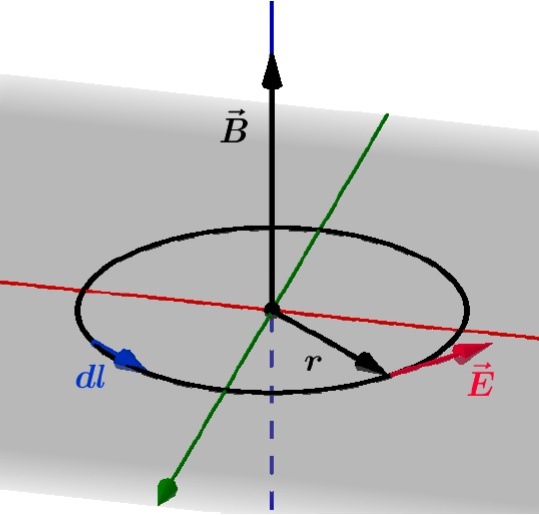
\includegraphics[width=0.6\textwidth]{./Figures/fig_s20}
	\caption{Momento sobre la órbita}
	\label{fig:s20}
\end{figure}


\begin{equation}
	\oint \V{E} \cdot \V{dl} = \oint E dl = \int \dPv{B}{t} \cdot d\V{S} = \dfrac{\partial}{\partial t} \int\V{B}\cdot d\V{S} = \dPv{B}{t}\pi r^{2}
\end{equation}

Como el campo es central, $E(r,t)$ entonces:

\begin{equation}
	E \oint dl = 2\pi rE = -\dP{B}{t}\pi r^{2}\rightarrow E= -\dfrac{r}{2}\dP{B}{t}
\end{equation}

Y en forma vectorial será:

\begin{equation}
	\V{E} = -\dfrac{1}{2}\V{r} \times \dPv{B}{t}
\end{equation}

Al introducir el campo magnético se crea una inhomogeneidad en el espacio y esta genera un campo eléctrico radial.

Sabemos que los electrones se encuentran en órbitas esféricas luego, como $\V{E} = -\dfrac{1}{2}\V{r} \times \dPv{B}{t}$ la fuerza que actúa sobre los electrones será:

\begin{equation}
	\V{f}_{i}= -e\V{E}(\V{r}_{i}) = -\dfrac{e}{2}\V{r}_{i} \times \dPv{B}{t} \quad \text{el valor medio será cero} \quad \langle\V{f}_{i} \rangle = 0
\end{equation}

calculemos la cupla que actúa sobre el material con $n$ electrones por átomo:

\begin{equation}
\begin{aligned}
&\dTv{L}{t}=\V{M}_{ext}= \langle \sum_{i} \V{r}_{i} \times \V{f}_{i} \rangle = -\dfrac{e}{2} \langle \sum_{i} \V{r}_{i} \times \left(  \V{r}_{i} \times \dP{B}{t} \hat{k} \right)   \rangle \\
&-\dfrac{ne}{2}\dP{B}{t}\left\langle \V{r} \times ( \V{r} \times \hat{k})\right\rangle =-\dfrac{ne}{2}\dP{B}{t}\left\langle \V{r}(\V{r}\cdot\hat{k})-\hat{k}(r^{2})\right\rangle\\
&=-\dfrac{ne}{2}\dP{B}{t}\left\langle \left[ (x\hat{i}+y\hat{j}+z\hat{k})z -\hat{k}(x^{2}+y^{2}+z^{2})\right]\right\rangle \\
&=-\dfrac{ne}{2}\dP{B}{t} \left[ <xz>\hat{i} + <yz>\hat{j} - <(x^{2}+y^{2})>\hat{k}  \right]\\
&=-\dfrac{ne}{2}\dP{B}{t} \left[ \dfrac{2}{3}<r^{2}>\hat{k}  \right]
\end{aligned}
\end{equation}










